%% Copernicus Publications Manuscript Preparation Template for LaTeX Submissions
%% ---------------------------------
%% This template should be used for copernicus.cls
%% The class file and some style files are bundled in the Copernicus Latex Package, which can be downloaded from the different journal webpages.
%% For further assistance please contact Copernicus Publications at: production@copernicus.org
%% https://publications.copernicus.org/for_authors/manuscript_preparation.html


%% Please use the following documentclass and journal abbreviations for preprints and final revised papers.

%% 2-column papers and preprints
\documentclass[gmd, manuscript]{copernicus}



%% Journal abbreviations (please use the same for preprints and final revised papers)


% Advances in Geosciences (adgeo)
% Advances in Radio Science (ars)
% Advances in Science and Research (asr)
% Advances in Statistical Climatology, Meteorology and Oceanography (ascmo)
% Annales Geophysicae (angeo)
% Archives Animal Breeding (aab)
% ASTRA Proceedings (ap)
% Atmospheric Chemistry and Physics (acp)
% Atmospheric Measurement Techniques (amt)
% Biogeosciences (bg)
% Climate of the Past (cp)
% DEUQUA Special Publications (deuquasp)
% Drinking Water Engineering and Science (dwes)
% Earth Surface Dynamics (esurf)
% Earth System Dynamics (esd)
% Earth System Science Data (essd)
% E&G Quaternary Science Journal (egqsj)
% European Journal of Mineralogy (ejm)
% Fossil Record (fr)
% Geochronology (gchron)
% Geographica Helvetica (gh)
% Geoscience Communication (gc)
% Geoscientific Instrumentation, Methods and Data Systems (gi)
% Geoscientific Model Development (gmd)
% History of Geo- and Space Sciences (hgss)
% Hydrology and Earth System Sciences (hess)
% Journal of Bone and Joint Infection (jbji)
% Journal of Micropalaeontology (jm)
% Journal of Sensors and Sensor Systems (jsss)
% Magnetic Resonance (mr)
% Mechanical Sciences (ms)
% Natural Hazards and Earth System Sciences (nhess)
% Nonlinear Processes in Geophysics (npg)
% Ocean Science (os)
% Polarforschung - Journal of the German Society for Polar Research (polf)
% Primate Biology (pb)
% Proceedings of the International Association of Hydrological Sciences (piahs)
% Scientific Drilling (sd)
% SOIL (soil)
% Solid Earth (se)
% The Cryosphere (tc)
% Weather and Climate Dynamics (wcd)
% Web Ecology (we)
% Wind Energy Science (wes)


%% \usepackage commands included in the copernicus.cls:
%\usepackage[german, english]{babel}
%\usepackage{tabularx}
%\usepackage{cancel}
%\usepackage{multirow}
%\usepackage{supertabular}
%\usepackage{algorithmic}
%\usepackage{algorithm}
%\usepackage{amsthm}
%\usepackage{float}
%\usepackage{subfig}
%\usepackage{rotating}


\begin{document}

\title{Constraining the historic carbon cycle in JULES-ES-1.0}

% \Author[affil]{given_name}{surname}

\Author[1,2]{Doug}{McNeall}
\Author[1]{Eddy}{Robertson}
\Author[1,2]{Andy}{Wiltshire}

\affil[1]{Met Office, FitzRoy Road, Exeter, EX1 3PB}
\affil[2]{College of Engineering, Mathematics, and Physical Sciences, University of Exeter, Exeter, EX4 4QE, UK}
\affil[3]{College of Life and Environmental Sciences, University of Exeter, Exeter, EX4 4RJ, UK}

%% The [] brackets identify the author with the corresponding affiliation. 1, 2, 3, etc. should be inserted.

%% If an author is deceased, please mark the respective author name(s) with a dagger, e.g. "\Author[2,$\dag$]{Anton}{Aman}", and add a further "\affil[$\dag$]{deceased, 1 July 2019}".

%% If authors contributed equally, please mark the respective author names with an asterisk, e.g. "\Author[2,*]{Anton}{Aman}" and "\Author[3,*]{Bradley}{Bman}" and add a further affiliation: "\affil[*]{These authors contributed equally to this work.}".


\correspondence{Doug McNeall (doug.mcneall@metoffice.gov.uk)}

\runningtitle{Constraining the historic carbon cycle in JULES-ES1.0}

\runningauthor{McNeall et al.}





\received{}
\pubdiscuss{} %% only important for two-stage journals
\revised{}
\accepted{}
\published{}

%% These dates will be inserted by Copernicus Publications during the typesetting process.


\firstpage{1}

\maketitle



\begin{abstract}

We constrain a large ensemble of JULES-ES-1.0 using modern observations of the carbon cycle. We explore the resulting constraint on the behaviour of the carbon cycle during the historical period.

We run Jules-ES-1.0 in a 500-member ensemble, driven by historical reanalysis. Each ensemble member has a different configuration of 32 input parameters, identified as potentially important in influencing land surface dynamics important by the  model developers. The parameters were perturbed randomly, in a Latin hypercube configuration, and within ranges defined by the model developers as being likely to at least produce output from the model.

We identify model variants, and their associated input configurations, where the model produces output that is consistent - within uncertain limits - with modern observations of the carbon cycle. We build statistical models of the relationship between the input configuration and the modern model output - termed emulators - which allow us to visualise and explore these relationships as if we had a much larger ensemble.

Using the ensemble and the emulators, we are able to generate a number of analyses that inform us of the drivers of model behaviour, and the source of model biases and errors. We provide a failure analysis, which allows us to identify parameter setting which cause failure of the model to run. We perform sensitivity analysis, which helps us quantify the effect of perturbing parameters on the model output.

Finding model outputs which match modern observations, we identify parts of input parameter space where the model output is acceptably good. We can rule out parameter settings where the output is not plausible. Constraining using each output in turn allows us to see which outputs are useful for constraining particular inputs. We see relationships between outputs manifest as joint constraint: when one output is used to constrain inputs, this induces a constraint on other, related outputs.

Having constrained both input parameter space and model outputs using modern observations of the carbon cycle, we examine the impact of the modelled carbon budget through time. What is the potential for constraining the carbon budget using only modern observations? What happens if we extend those observations back through time?

Our analysis informs the construction a new ensemble design, with ensemble members picked to lie within the input space not ruled out by a comparison of the model behaviour with modern observations. 
\end{abstract}


\copyrightstatement{TEXT} %% This section is optional and can be used for copyright transfers.

\section{Analysis plan}

Our guiding principles for this paper: what does comparing the model output with observations tell us about where to run the model, and also about the history of the carbon cycle?

Suggested paper structure
\begin{enumerate}
    \item Introduction. Motivation
    \item Ensemble
\end{enumerate}

An extension to consider: what happens when we project the constrained space forwards through time. For this, we need runs using future boundary conditions.


\introduction  %% \introduction[modified heading if necessary]

\begin{enumerate}
    \item Jules version, aims, context 
    \item Uncertainty Quantification for model development
\end{enumerate}



\section{JULES behaviour across the ensemble}

\subsection{Ensemble design}

\subsection{Failure analysis}

We analyse the ensemble to remove "failed" runs, and remove ensemble members in parts of parameter space that cannot hope to produce a useful simulation of the carbon cycle. First, we map ensemble members where the model crashed or failed to run, perhaps due to numerical error (termed "failed"). Second, we identify parts of parameter space where important parts of the carbon cycle are completely missing - that is, basic carbon cycle quantities are at or close to zero at the end of the run (termed "zero carbon cycle"). For this second class, we choose a threshold of mean modern global NPP close to zero (* scale data to find out)

The nature of perturbed parameter ensembles is that there is often a setting of some parameters that makes up for a poor choice of a particular parameter, and so outright and easily identifiable thresholds for failure in the marginal range of a particular parameter are rare. However, careful visualisation and analysis can give the modeller a good idea of regions of parameter space that can be removed, or parameters that the model is particularly sensitive to.

in fig. \ref{fig:run-failure-pairs}, we see a pairs plot of "failed" runs (upper right panels) and, "zero carbon cycle" panels (lower left panels). The plot shows the two-dimensional projections of run failures against each pair of inputs, allowing visual identification of inputs that control failures, and any potential two-way interactions.

For example, we can see that both $f0\_io$ and $b\_wl\_io$ have important thresholds, beyond which there is almost no chance of a functioning carbon cycle. As there appears little to no interaction between these two, this presents as a nearly-blank plot at the intersection of the parameters on the plot, with inputs identifying zero-carbon runs around the edges of the sub plot.


Combine the plot for these two? - pairs of both failures and $f0\_io b\_wl\_io$ threshold?

\begin{figure*}[t]
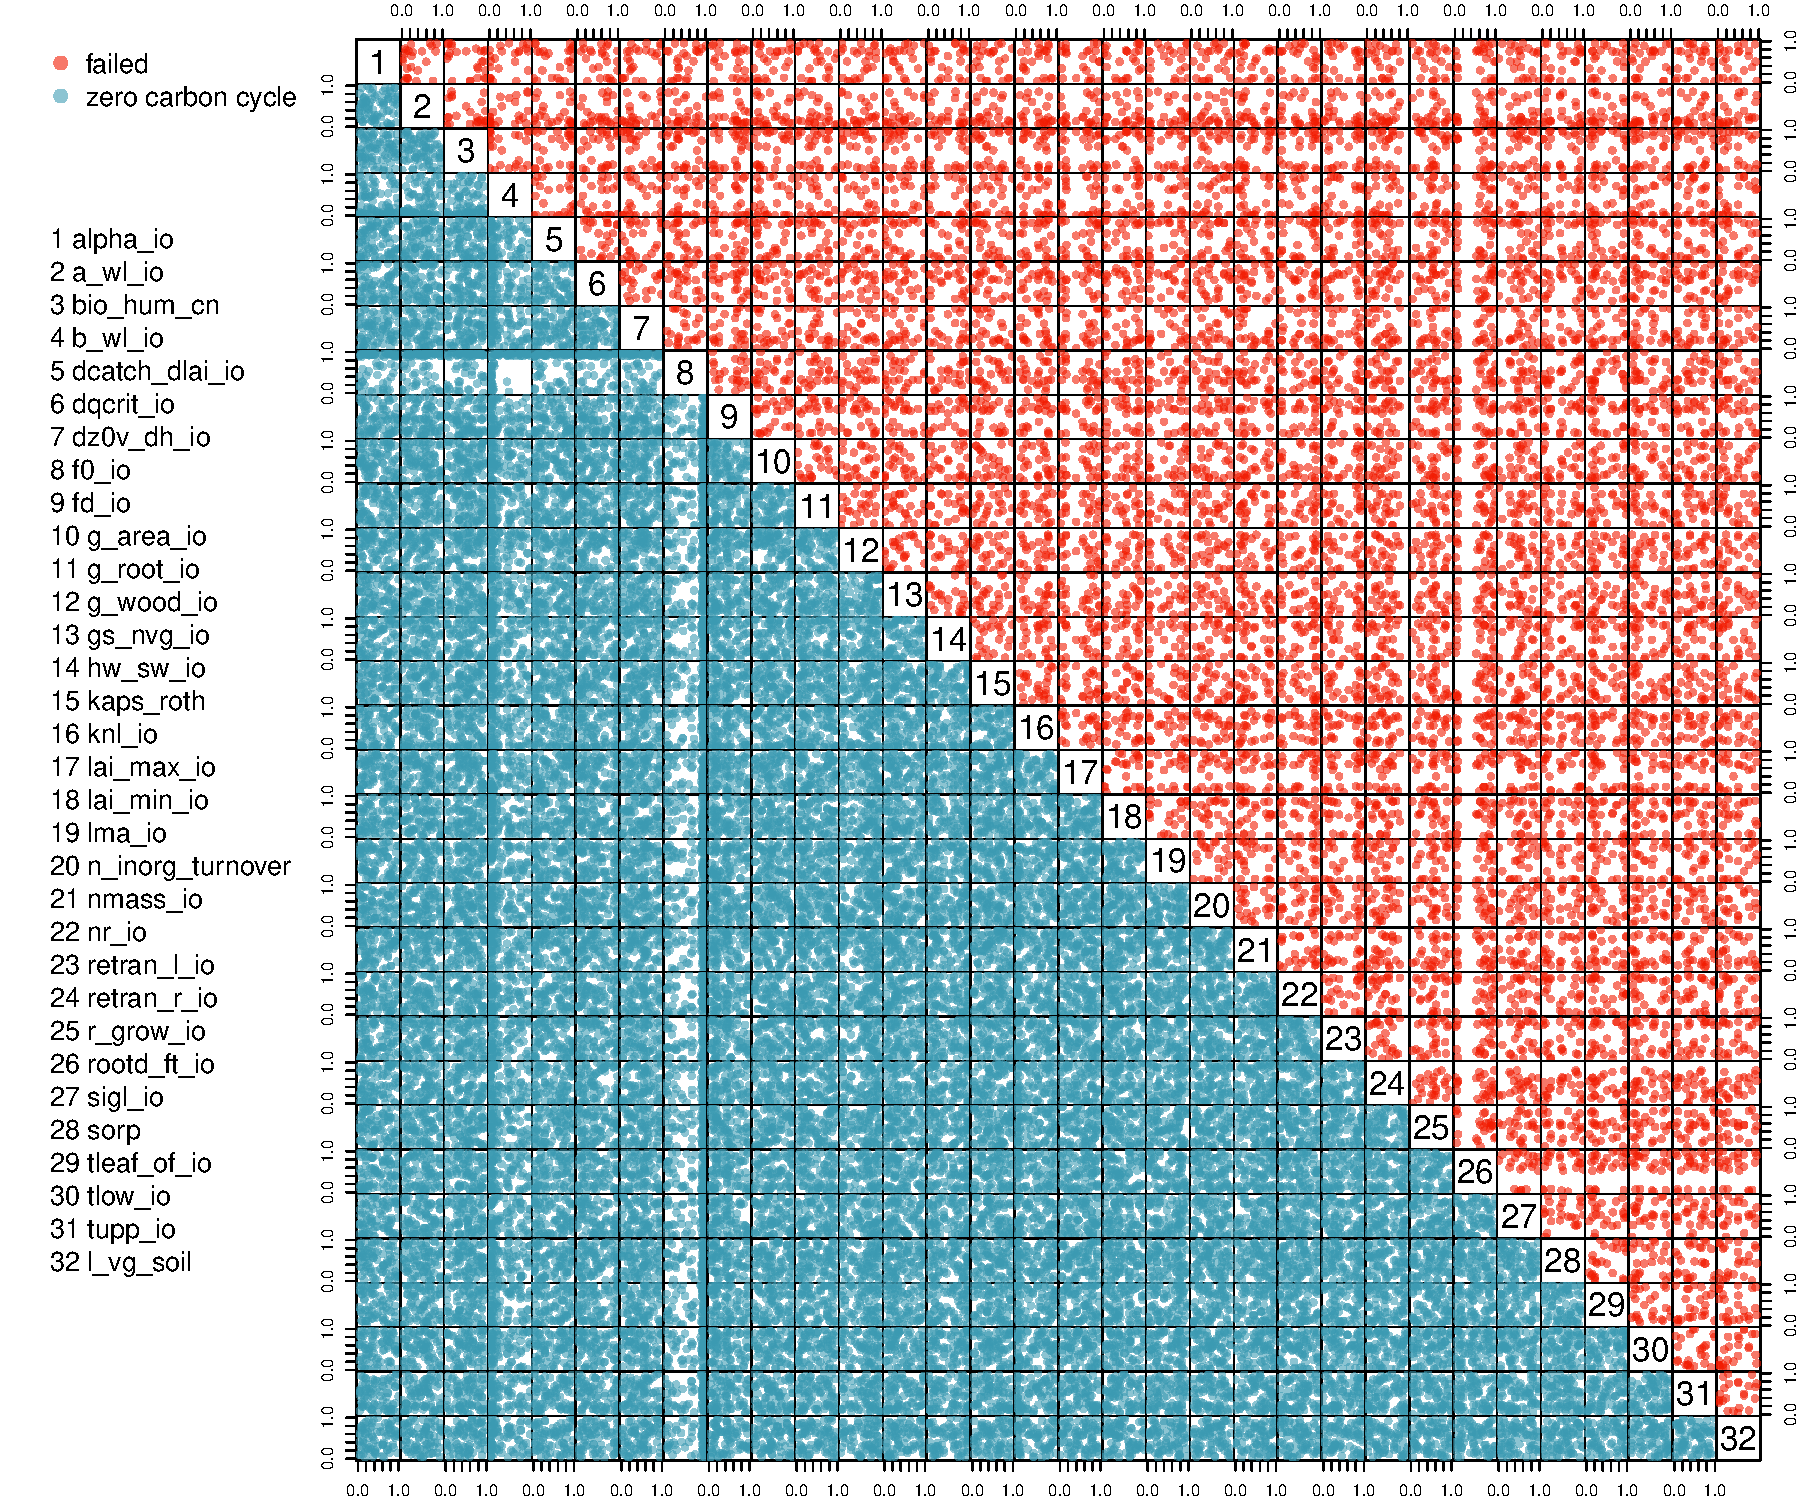
\includegraphics[width=12cm]{./graphics/run-failure-pairs.pdf}
\caption{Pairs plot of the locations in (normalised) input space of the ensemble members that did not run/failed.}
\label{fig:run-failure-pairs}
\end{figure*}


\begin{figure*}[t]
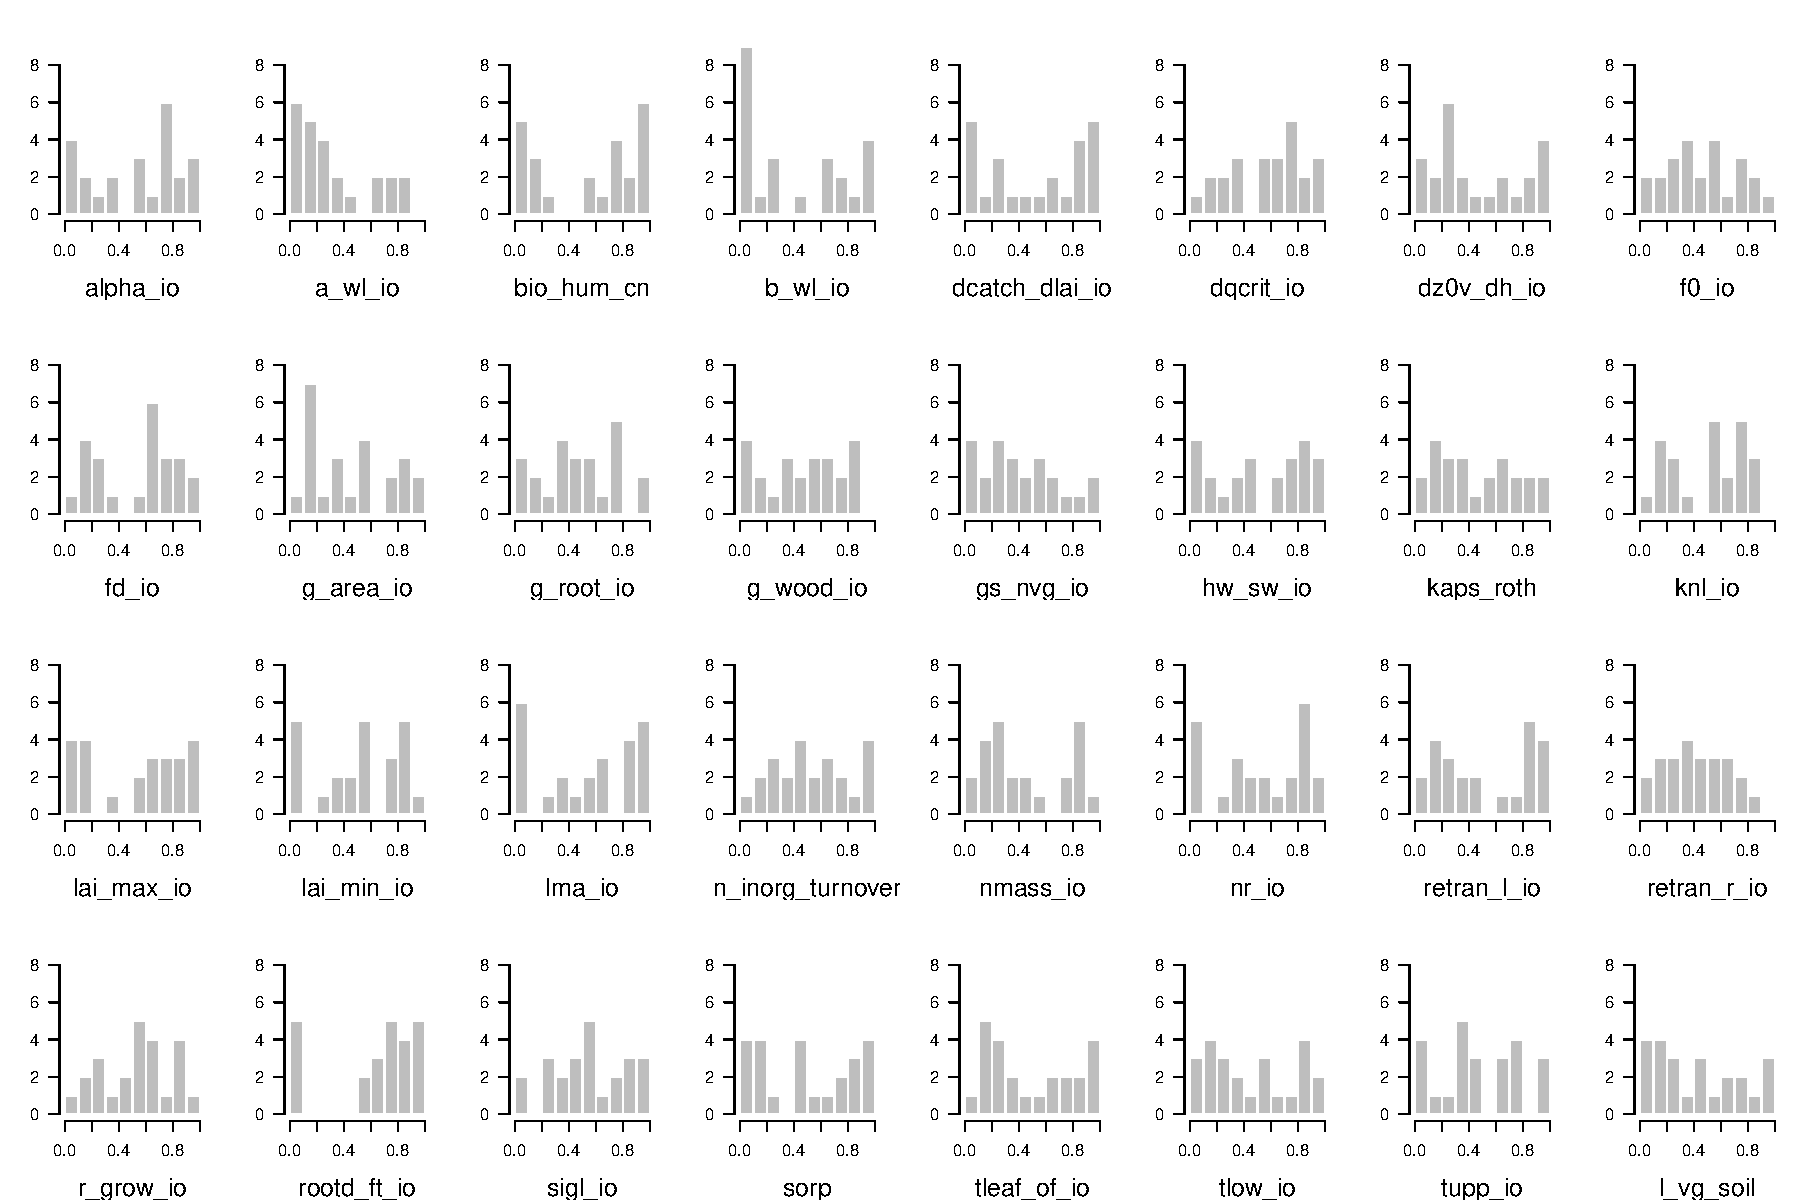
\includegraphics[width=12cm]{./graphics/run-failure-hists.pdf}
\caption{Histograms of the locations in (normalised) input space of the ensemble members that did not run/failed.}
\end{figure*}



%%% TWO-COLUMN FIGURES
%
%%f
\begin{figure*}[t]
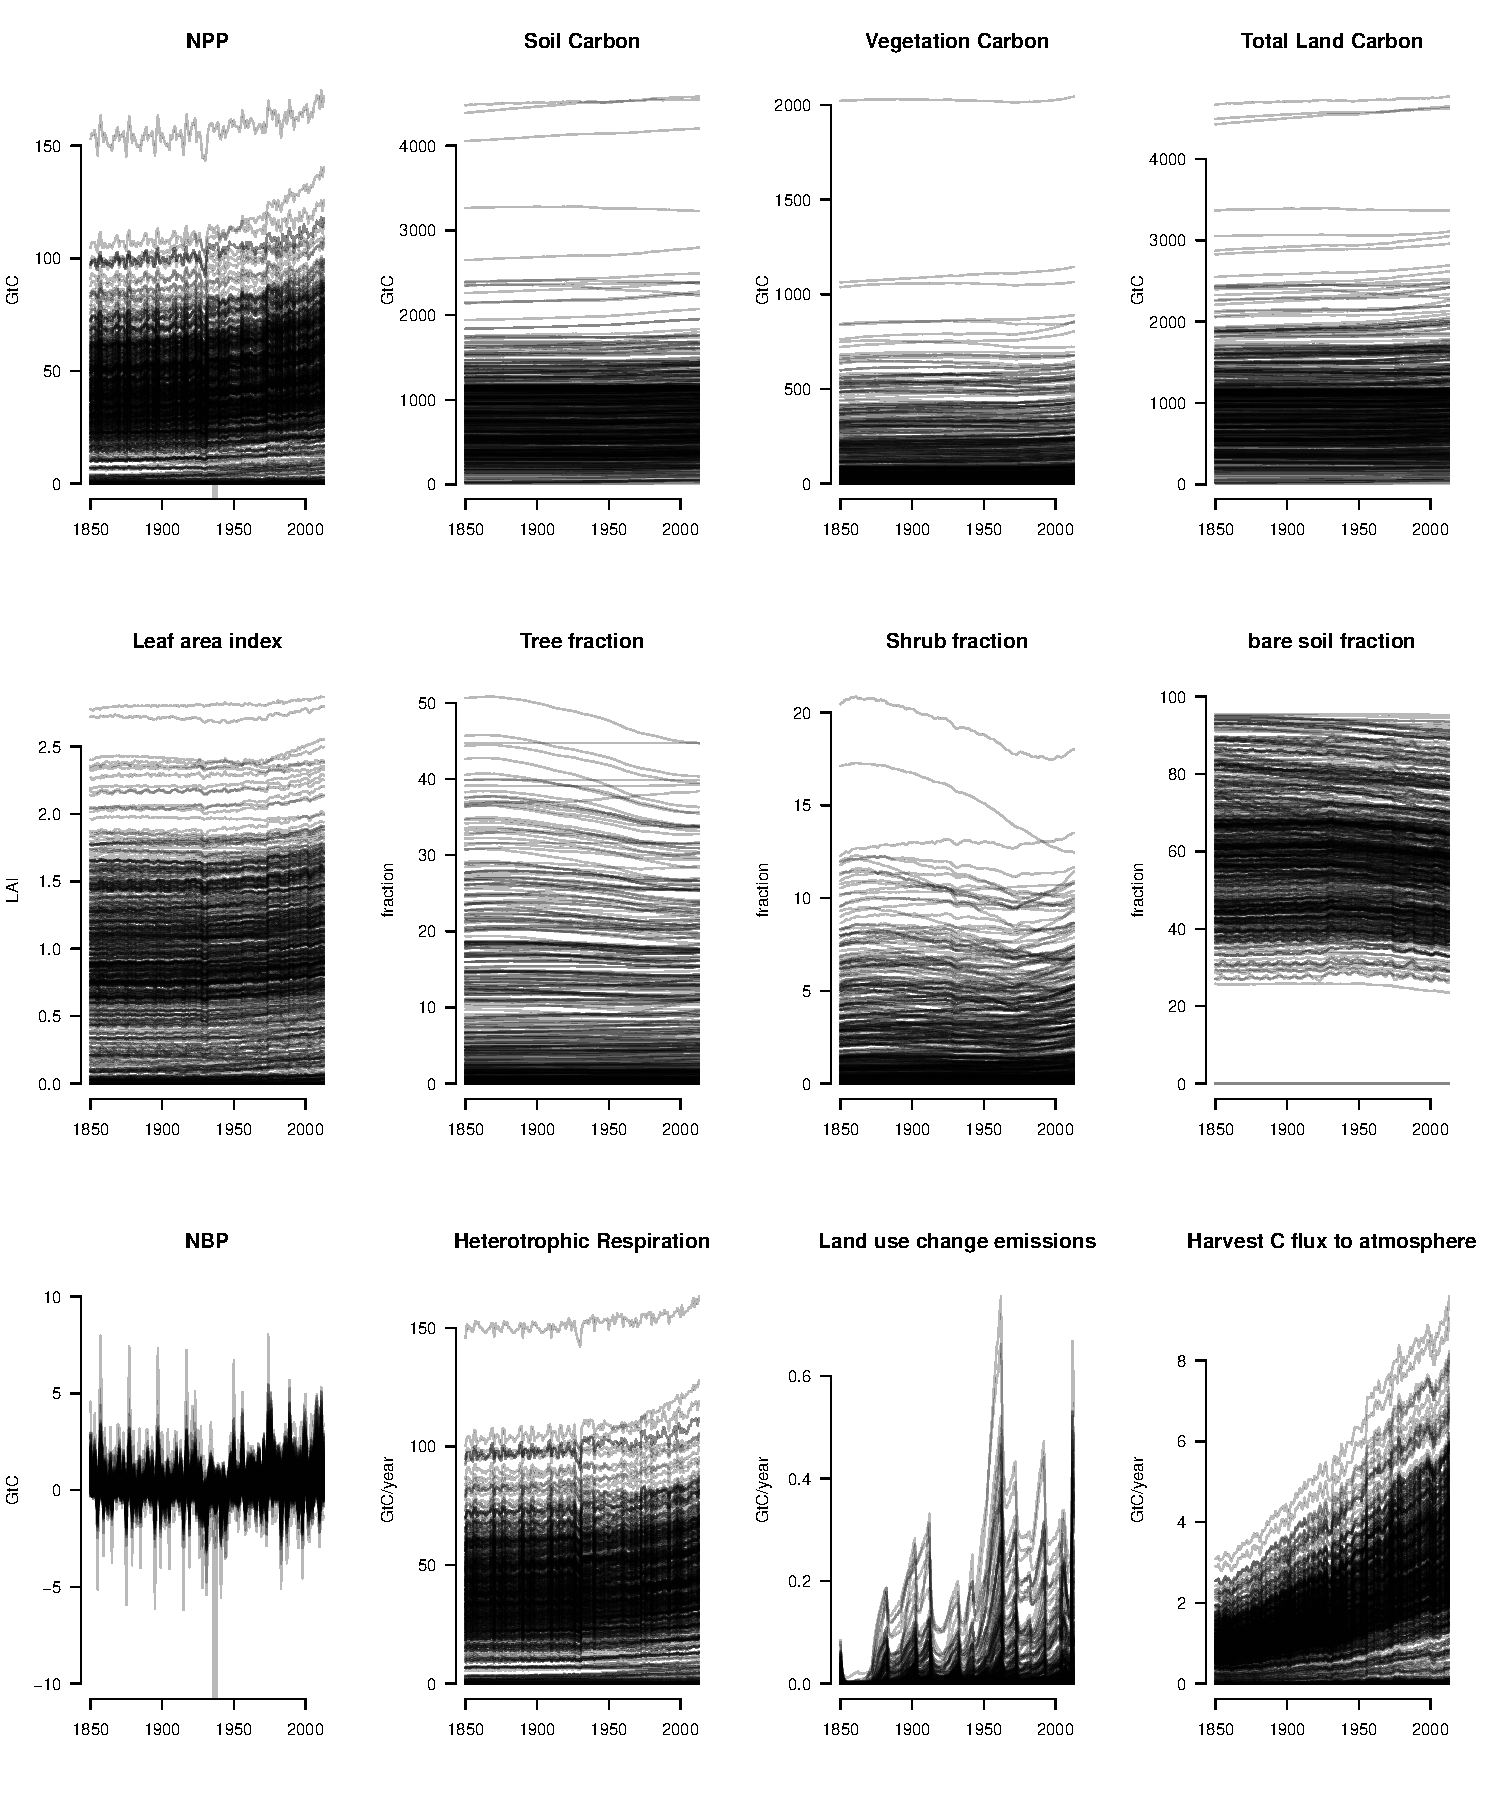
\includegraphics[width=12cm]{./graphics/plot-carbon-cycle-timeseries-primary-1.pdf}
\caption{Primary carbon cycle quantities in the JULES ensemble.}
\end{figure*}


%%% TWO-COLUMN FIGURES
%
%%f
\begin{figure*}[t]
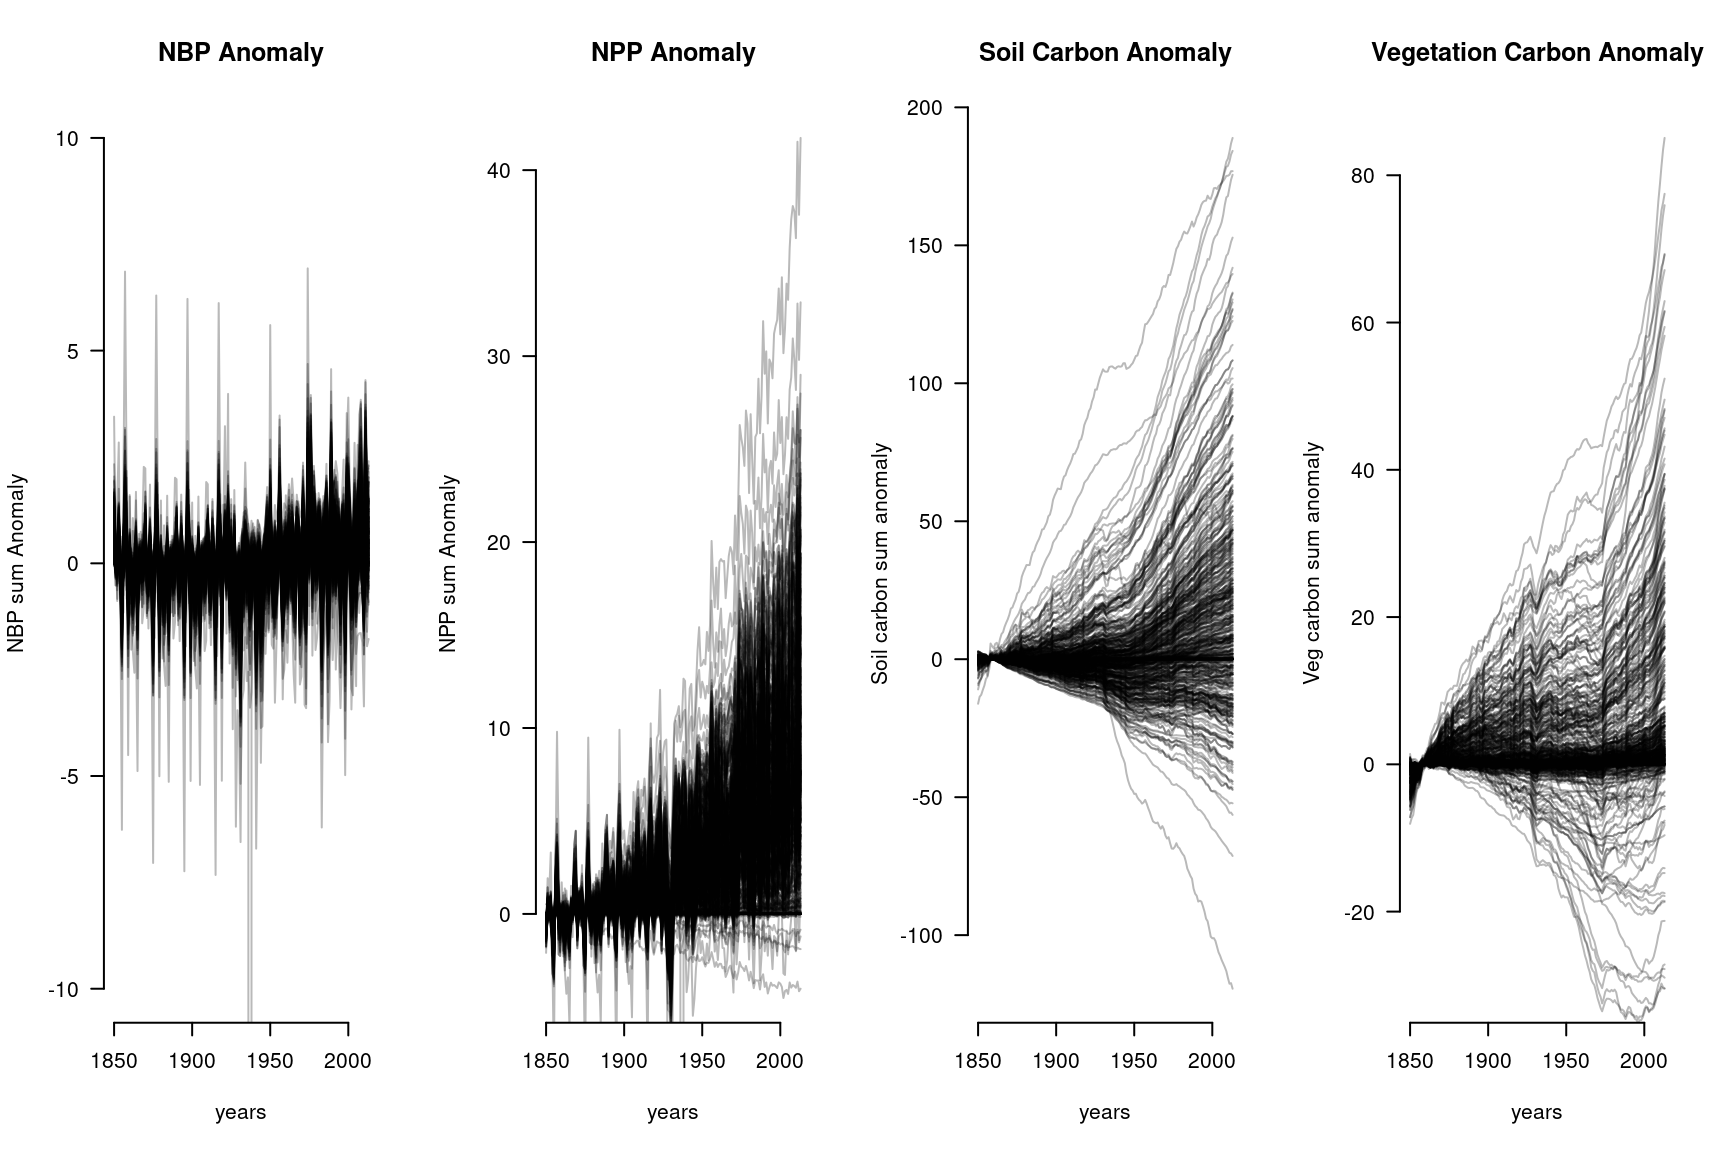
\includegraphics[width=12cm]{./graphics/plot-carbon-cycle-anomaly-timeseries-1}
\caption{Carbon cycle quantities in the JULES ensemble.}
\end{figure*}





\section{What we need to take the next steps in the analysis}

\begin{itemize}
    \item Modern observations corresponding to model outputs.
    \item Expert-derived limits using above.
    \item CMIP6 boundaries of above.
    \item Model outputs (through time) we'd like to include (regional forest fraction, atmospheric carbon growth, total land carbon).
\end{itemize}

\begin{enumerate}
    \item 
\end{enumerate}



\section{Results}



\subsection{Sensitivity Analysis}
We use the emulator fit to a range of outputs to perform several types of sensitivity analysis.

\subsubsection{Global one-at-a-time Sensitivity}

A one-at-a-time (OAAT) sensitivity gives a simple and easy-to-interpret measure of the impact of each input on a variety of outputs, but does not include the effects of any interactions between inputs (for example, a non-linear change in model outputs as two or more inputs vary together).  

A one-at-a-time analysis can be completed with a relatively small number of model runs - for example, a low, middle and high run for each parameter in our 32 input dimension example would take fewer than 100 runs. However, using an emulator allows us to better characterise the response of the model across the entire sweep of each parameter.

We fit a gaussian process emulator (direct km) to each global summary output, both as a ``modern value'' (mean of 1994 - 2014), and as an ``anomaly" (change since 1850-1870).

We sample from the input space in a one-at-a-time fashion: each input is sampled uniformly across it's input space, with all other inputs held at median values. The variance of the mean emulated output as each input is varied is then used as a measure of the sensitivity of that output to the corresponding input. Variance is used as opposed to magnitude of change, as we expect some model outputs not to rise or fall monotonically as an input varies.

Different model outputs are clearly sensitive to different model inputs, and so we also seek ways of summarising sensitivity across model outputs. One method is simply to find the mean effect across model outputs. Sensitivities are normalised so that they lie in a $[0 -1]$ range for each output. Summary measures for each input are then averaged across all outputs, and the plotted inputs are ranked by their average influence across all outputs. Individual sensitivities and summaries can be seen in fig. \ref{fig:oat_var_sensmat_level1a_Y} for the modern value, and in fig. \ref{fig:oat_var_sensmat_level1a_YAnom} for the change over the historic period of the ensemble. 

\subsubsection{FAST sensitivity analysis}

We use Fourier Amplitiude Sensitivity Test (FAST) as a further measure of global sensitivity of the model outputs to its inputs. The test is administered as the FAST99 algorithm of \cite{Saltelli1999}, through the R package Sensitivity \citep{Rsensitivity}. Again, this algorithm requires a large number of model runs, and so we use emulated model outputs in place of dedicated model runs. This comes at the cost of a risk of innacuracy, as the emulated model outputs won't perfectly reproduce the true model runs at the corresponding inputs. However, the emulator is shown to work adequately for the model outputs in section \ref{ssec:emulator_accuracy}. 

\subsubsection{Choosing or excluding inputs}


If we were asked to decide which parameters to exclude a set of parameters for a new ensemble, which would we choose? One way to choose might be to exclude those parameters which have little effect on \emph{any} model output of interest. For this ensemble we find these by ranking the inputs by their summarising their OAAT effect across all outputs. Choosing the inputs that are consistently ranked lowest would be a conservative method of excluding inputs.


%t
\begin{table*}[t]
\caption{Ranking sensitivity to inputs}
\label{table:sens_rank_total}
\begin{tabular}{l r r r r r}
\tophline
parameter & OAT modern value & FAST modern value & OAT anomaly & FAST Anomaly & highest rank \\ 
\middlehline
alpha\_io            &            1          &       1      &      1      &       1    &     1 \\ 
b\_wl\_io              &            2        &          2     &       3   &          2    &     2 \\ 
lai\_max\_io           &            4      &             6    &        2    &         3    &     2 \\ 
g\_area\_io            &            3      &            7     &       5   &          6    &      3 \\ 
n\_inorg\_turnover     &            6      &            3     &       4     &        4    &     3 \\ 
fd\_io                &            5      &            4     &       6   &          5    &     4 \\ 
lma\_io               &            7      &            5     &      15     &       13    &     5 \\ 
nmass\_io             &            9      &            9     &       8      &       7    &     7 \\ 
r\_grow\_io            &            8      &            8     &       7       &      8    &     7 \\ 
a\_wl\_io              &           11      &           10     &      11       &      9    &     9 \\ 
bio\_hum\_cn           &           26      &           27     &       9   &         10    &     9 \\ 
dqcrit\_io            &           10      &           11     &      18   &         16    &    10 \\ 
tupp\_io              &           18      &           18     &      10   &         11    &    10 \\ 
lai\_min\_io           &           14      &           14     &      13 &           12    &    12 \\ 
tleaf\_of\_io          &           12     &            12     &      12   &         14    &    12 \\ 
kaps\_roth            &           13      &           13     &      19    &        18    &    13 \\ 
hw\_sw\_io             &           15      &           16     &      14     &       15    &    14 \\ 
rootd\_ft\_io          &           17      &           15     &      22  &          21    &    15 \\ 
f0\_io                &           16      &           17     &      17   &         17    &    16 \\ 
retran\_l\_io          &           20      &           21     &      16   &         19    &    16 \\ 
dz0v\_dh\_io           &           19      &           19     &      27    &        25    &    19 \\ 
g\_root\_io            &           21      &           20     &      23     &       23    &    20 \\ 
g\_wood\_io            &           22      &           25     &      21  &          20    &    20 \\ 
nr\_io                &           23      &           23     &      20   &         22    &    20 \\ 
gs\_nvg\_io            &           30      &           22     &      26    &        24    &    22 \\ 
dcatch\_dlai\_io       &           27      &           24     &      30    &        31    &    24 \\ 
tlow\_io              &           24      &           32     &      24    &        29    &    24 \\ 
l\_vg\_soil            &           25      &           29     &      25    &        26    &    25 \\ 
retran\_r\_io          &           28      &           26     &      29    &        27    &    26 \\ 
sigl\_io              &           32      &           30     &      28    &        30    &    28 \\ 
sorp                 &           29      &           28     &      31    &        28    &    28 \\ 
knl\_io               &           31      &           31     &      32       &     32    &    31 \\ 

\bottomhline
\end{tabular}
\belowtable{} % Table Footnotes

\end{table*}



\begin{figure*}[t]
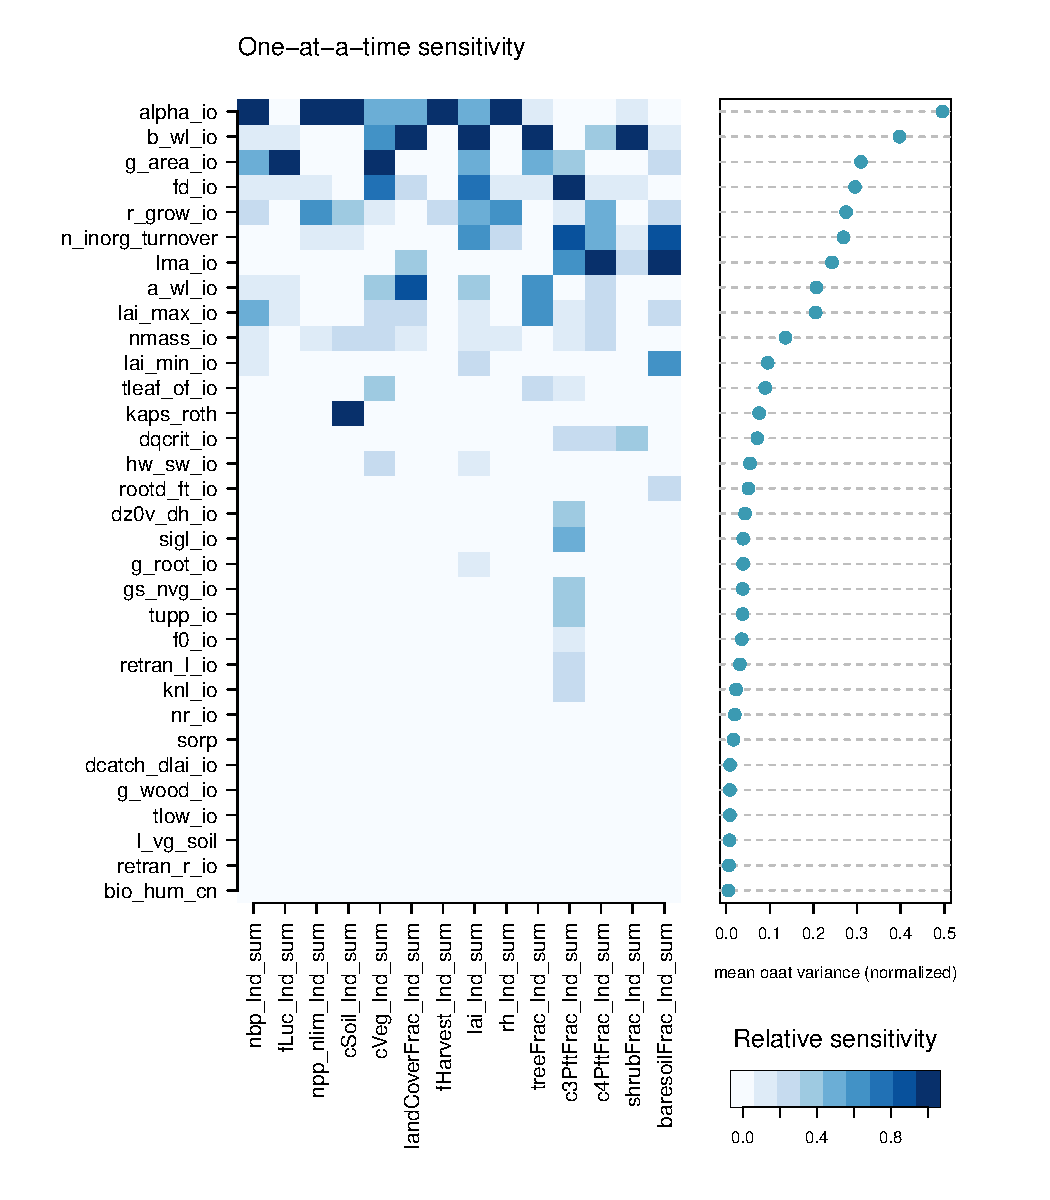
\includegraphics[width=12cm]{./graphics/oat_var_sensmat_level1a_Y}
\caption{One-at-a-time sensitivity summary for global summary ``modern value" output.}
\label{fig:oat_var_sensmat_level1a_Y}
\end{figure*}

\begin{figure*}[t]
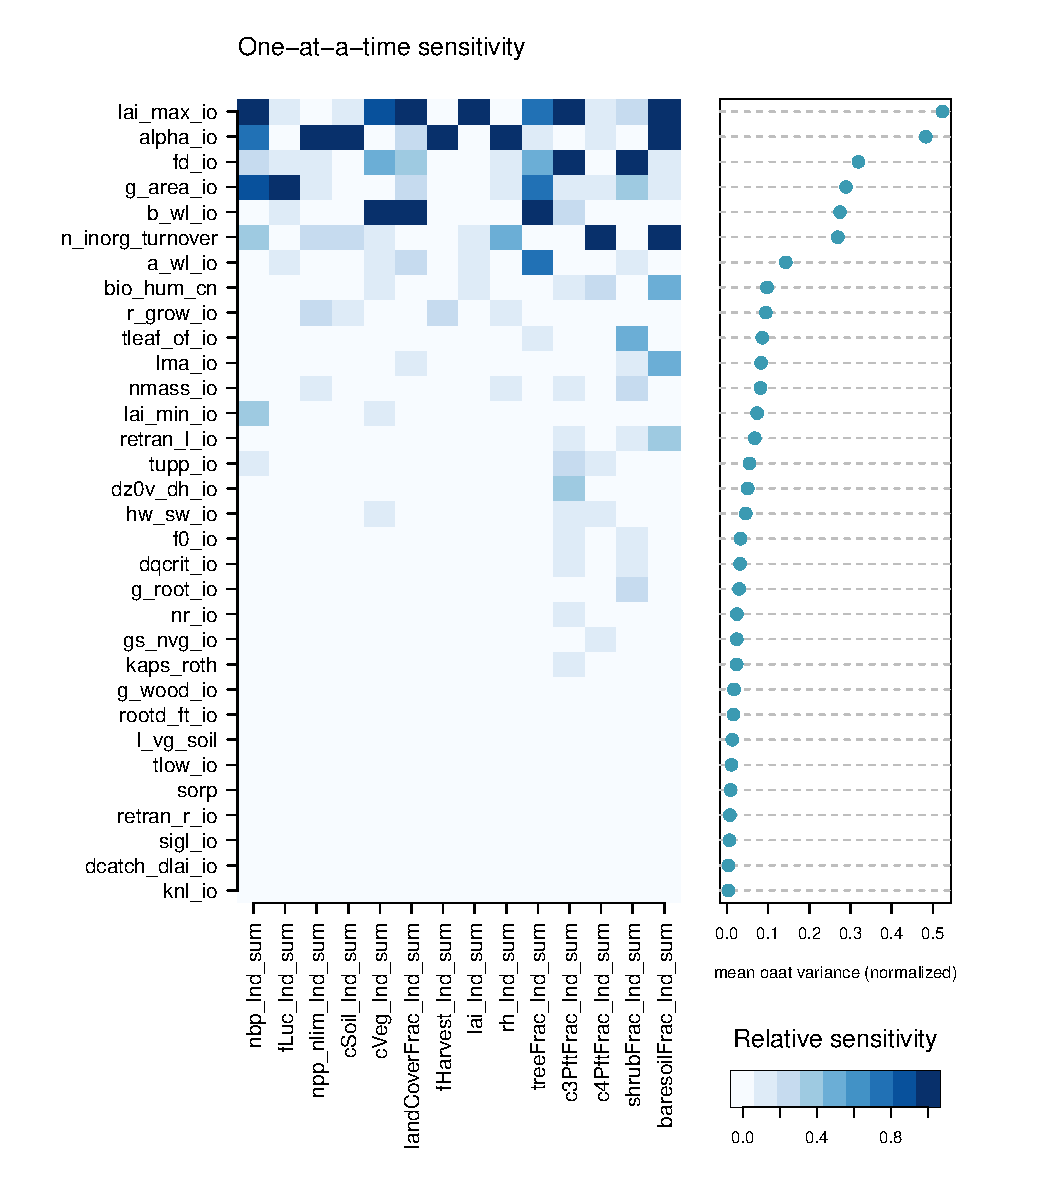
\includegraphics[width=12cm]{./graphics/oat_var_sensmat_level1a_YAnom}
\caption{One-at-a-time sensitivity summary for global summary ``anomaly" (change since 1850-1870) output.}
\label{fig:oat_var_sensmat_level1a_YAnom}
\end{figure*}


\subsubsection{Sensitivity of constraint outputs}

We add detail to our one-at-at-time sensitivity of important outputs - those that we use for constraining JULES. We plot the emulated mean of the each of four outputs - NBP, NPP, vegetation carbon and soil carbon, as each parameter in increased from its minimum to maximum range.

\begin{figure*}[t]
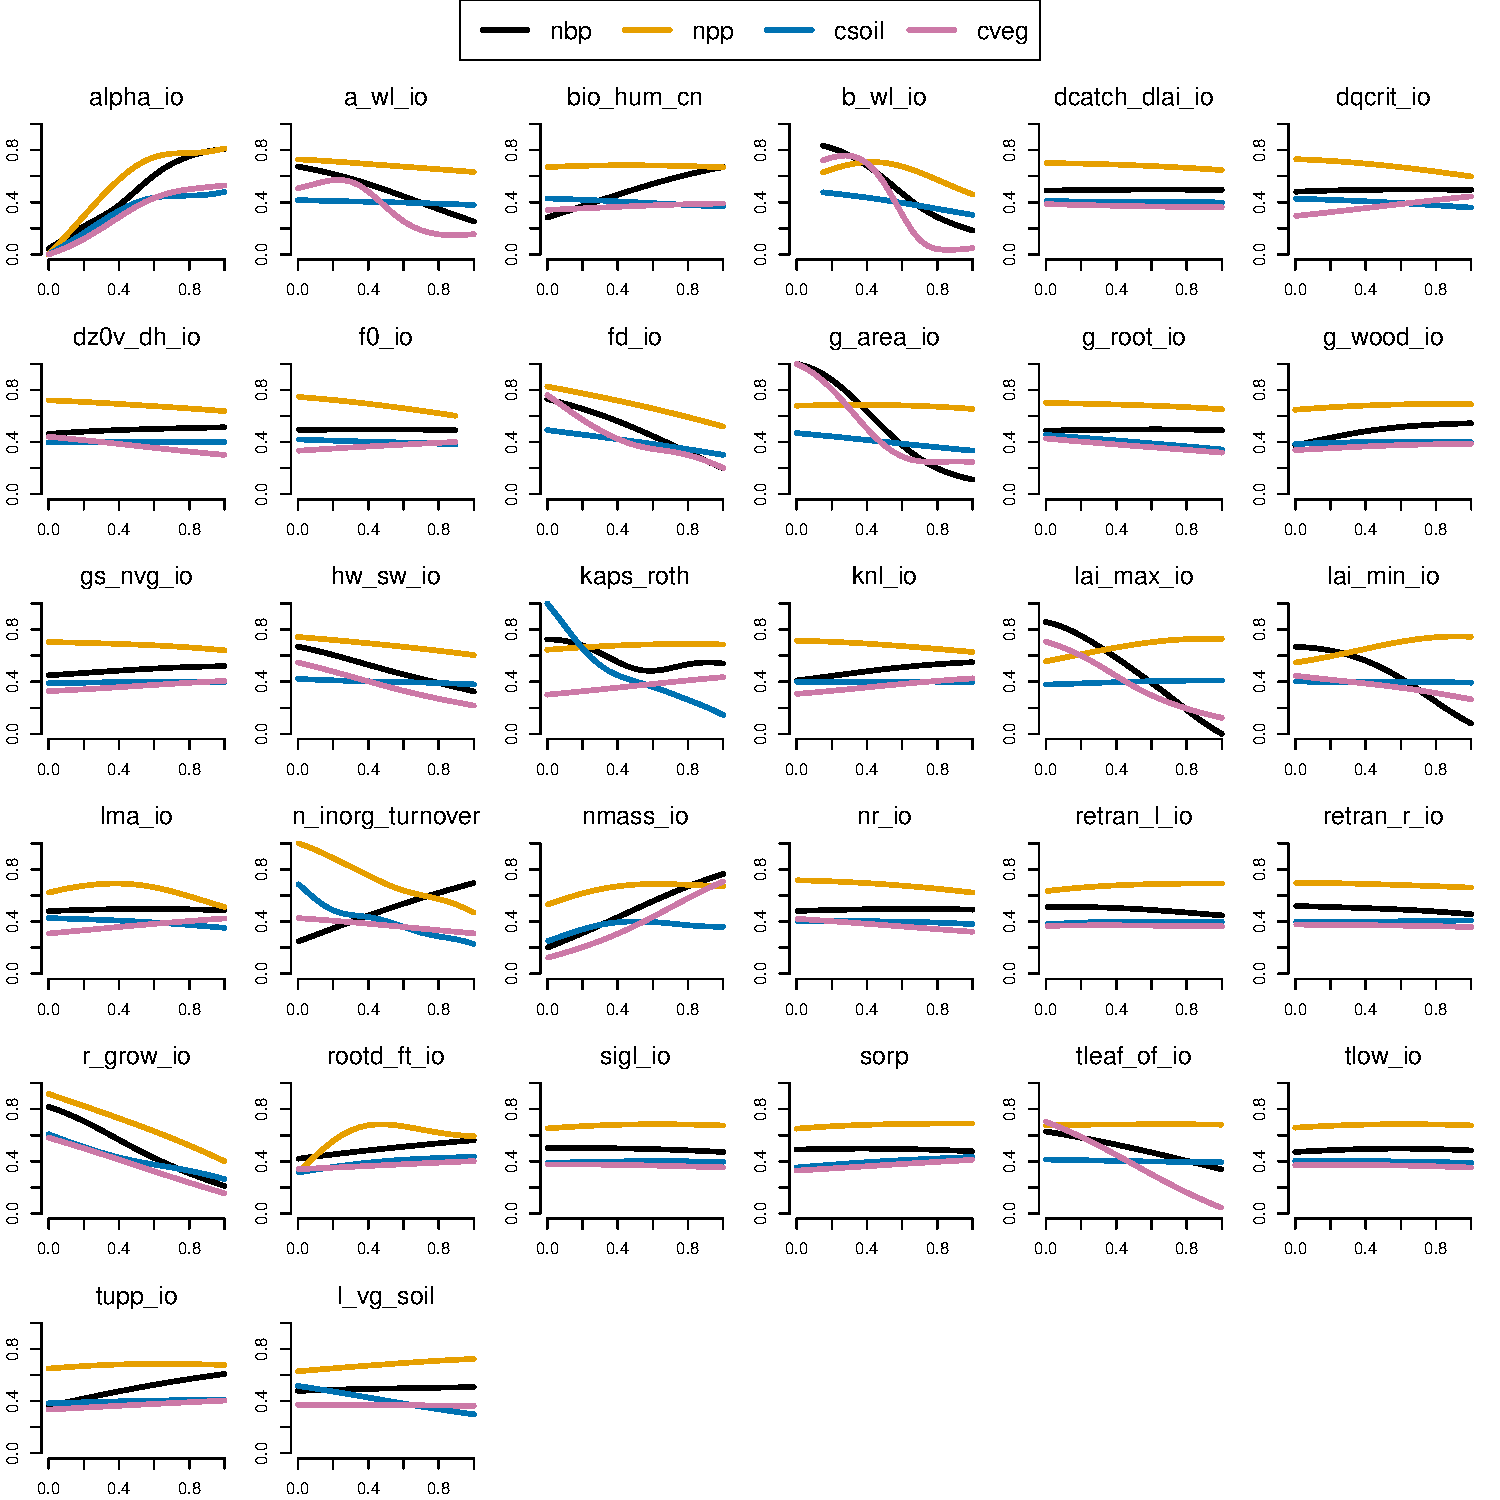
\includegraphics[width=12cm]{./graphics/Y_oaat_const_level1a_scaled_norm}
\caption{One-at-a-time sensitivity summary for global summary of the ``modern value" of the constraint variables (nbp, npp, cVeg, cSoil)}
\label{fig:Y_oaat_const_level1a_scaled_norm}
\end{figure*}



\subsection{Constraining the historical carbon cycle}

We can constrain both the historical behaviour of the model and the model parameter input space by comparison of the model behaviour with observations and other model simulations.

We use a number of strategies for model constraint.

We find the most effective outputs for constraining model inputs and behaviour. ** One at a time constraint analysis, needs doing **


\subsubsection{Direct constraint of ensemble members}

The simplest way to constrain the historical behaviour of the carbon cycle is by removing from the ensemble model runs that lead to implausible values of basic carbon cycle quantities in the modern era. These constraints are outlined in table \ref{table:level_2_constraints}.

Our strategy is to exclude model variants that have soil or vegetation carbon stocks, net primary production (NPP) or net biome production (NBP) in the modern era that are inconsistent with modern observations or understanding. This approach borrows from the more formal process of history matching, in that ensemble members deemed implausible are excluded. In history matching, a formal statistical process is used, whereas in this first section, we are concerned with simply removing a number of very poorly behaving model variants, such that the modeller is certain that they don't offer useful information about the carbon cycle.

A challenge when comparing models of the land surface with the carbon cycle is the lack of model-independent observations back through time, and the relatively large uncertainty in comparing the model dynamics with the true behaviour of the system. Because of this, it is important to be tolerant to a wide range of behaviours in the model itself. 

The modeller (Wiltshire) gave ranges for Vegetation and Soil carbon stocks, NBP and NPP at the end of the model run (2013), with instruction to be conservative - that is with enough range to be sure to encompass any reasonable uncertainties (see table \ref{table:level_2_constraints}). These ranges were considerably wider than the ranges given by the AR5, for example.

Because of this wide tolerance of modern behaviours, we perhaps should not be too optimistic that large regions of input space, or potential histories of the carbon cycle, should be excluded (alternatively that the space of possible histories and input space should be overly constrained).

However, even given the wide ranges of tolerable behaviour, a large number of our ensemble members are excluded. Of the 362 ensemble members that run, and have non-zero carbon cycle properties (constraint level 1a), only 37 (10.2\%) fall within the wide bounds set by the modeller.

%% TWO-COLUMN TABLE
%%% The different columns must be seperated with a & command and should
%%% end with \\ to identify the column brake.

%t
\begin{table*}[t]
\caption{Level 2 output constraints}
\label{table:level_2_constraints}
\begin{tabular}{l r r}
\tophline
Constraint & Minimum & Maximum \\ 
\middlehline
NBP & 0 GtC/yr &  10 GtC/yr\\
NPP & 35 GtC/yr & 80 GtC/yr \\
Soil Carbon stock & 750 GtC &  3000 GtC\\ 
Vegetation Carbon stock & 300 GtC & 800 GtC \\

\bottomhline
\end{tabular}
\belowtable{} % Table Footnotes

\end{table*}

\begin{figure*}[t]
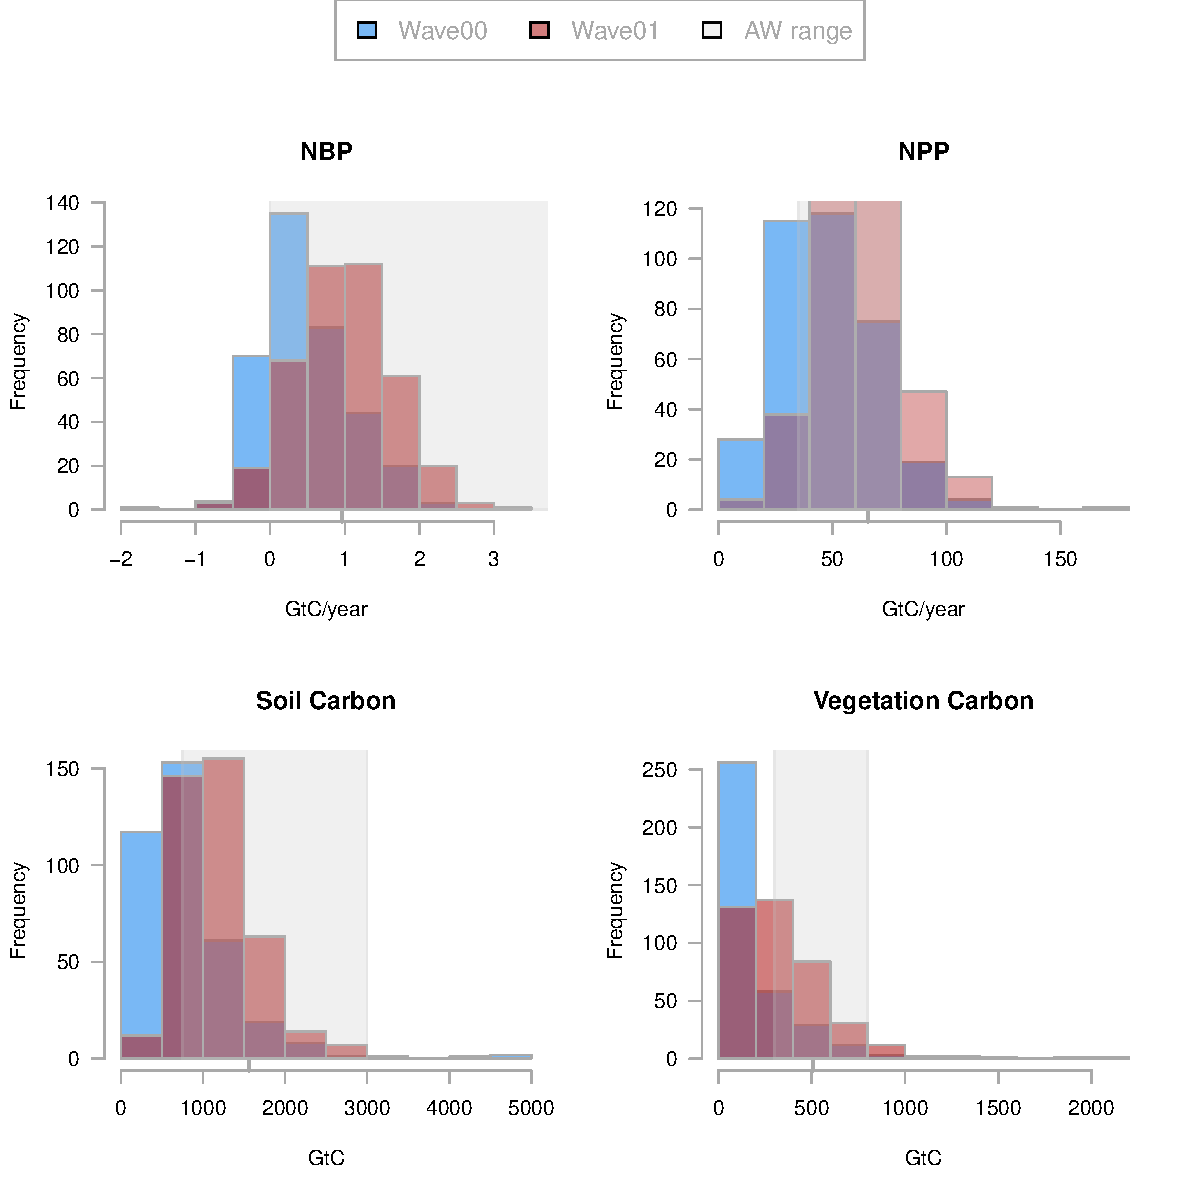
\includegraphics[width=12cm]{./graphics/level_2_constraints_hists.pdf}
\caption{level 1 constraint histograms}
\label{fig:level_2_constraints_hists}
\end{figure*}


\subsection{Constraining input space with an emulator}

Constraining the ensemble my directly rejecting implausible members gives us a useful but rough outline of the input space where the model might be said to behave "well". With only 37 ensemble members, we are able to outline the valid 32 dimensional input space only very approximately. For example the pairs plot in figure \ref{} shows the two-dimensional projections of the retained ensemble members, and more densely populated regions show where the model is more likely to produce valid output.

\begin{figure*}[t]
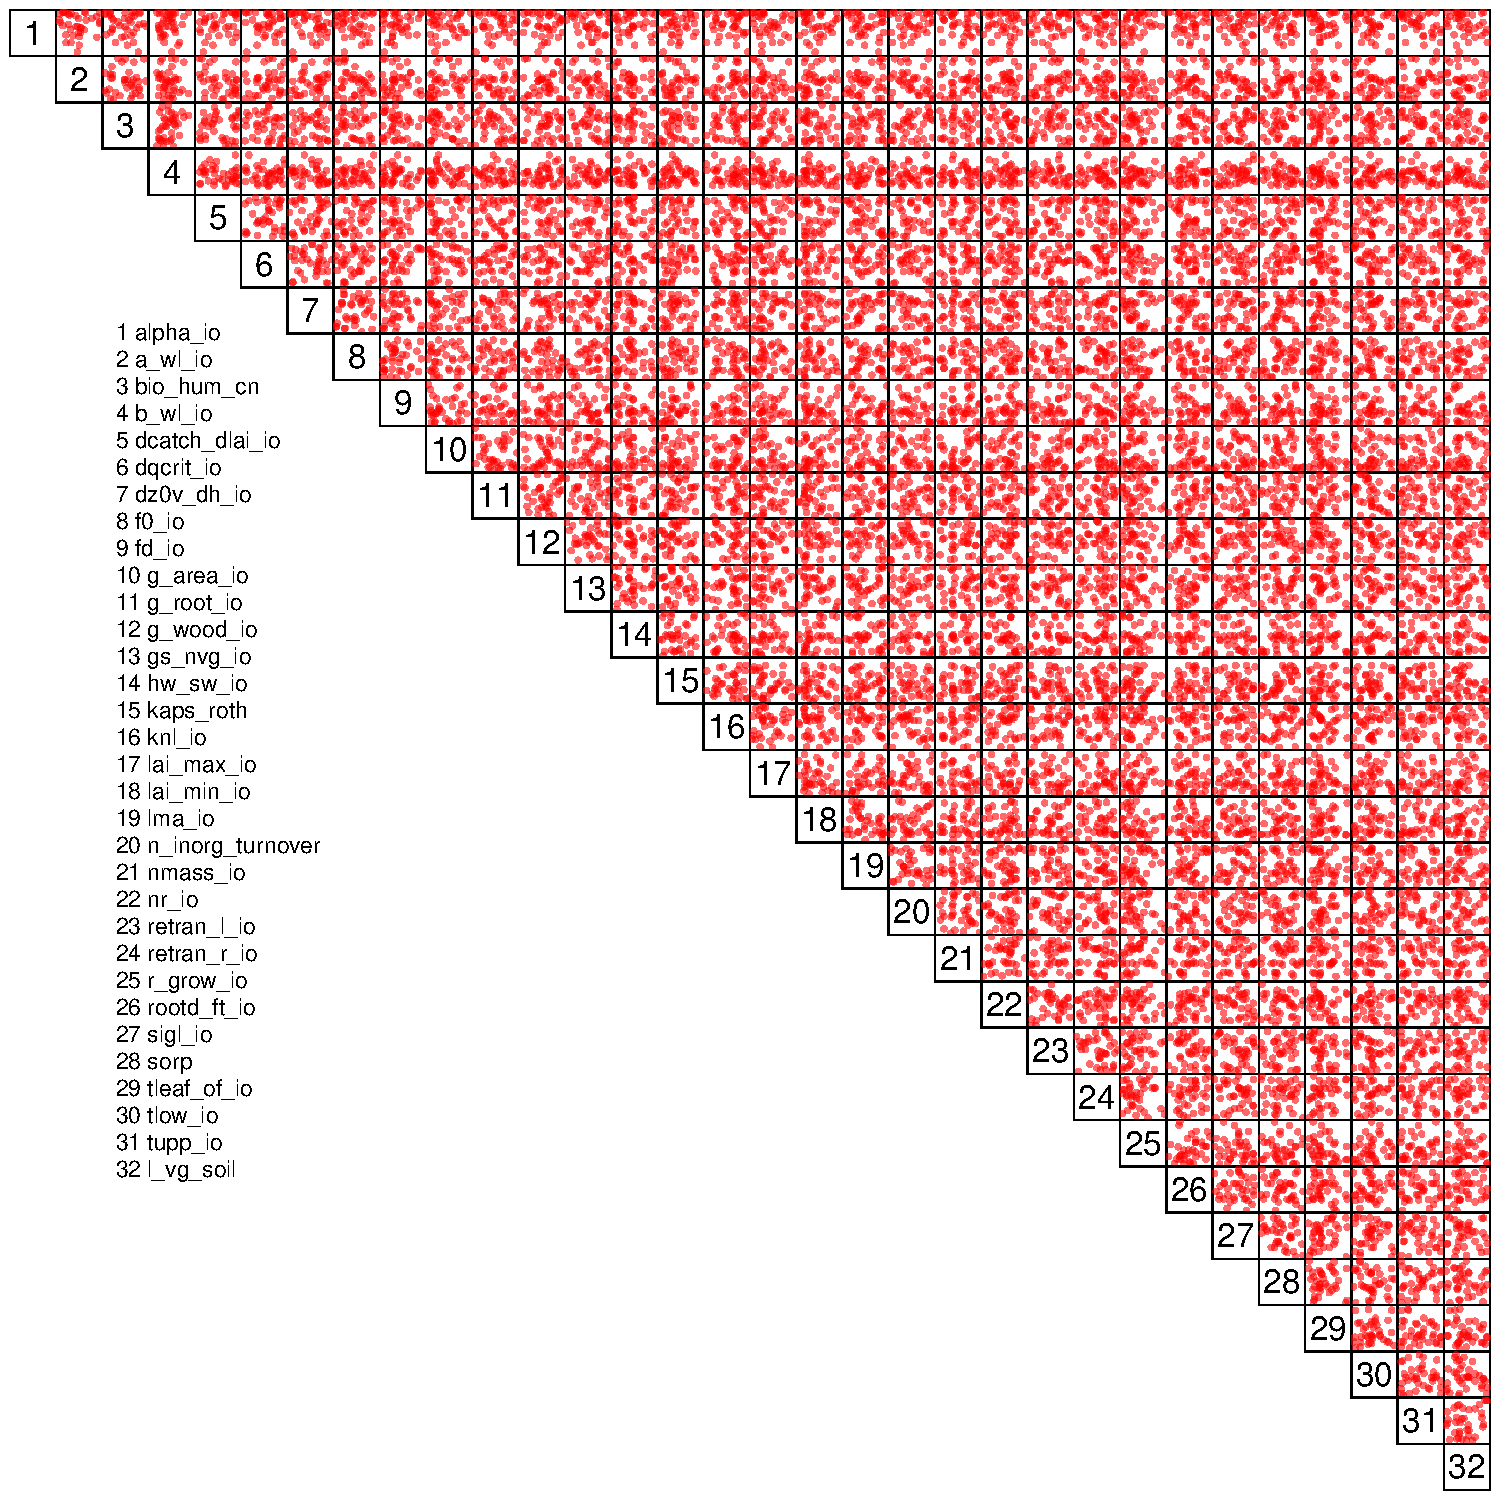
\includegraphics[width=12cm]{./graphics/pairs_level2_inputs.pdf}
\caption{level 2 pairs density plot.}
\label{fig:pairs_level2_inputs}
\end{figure*}

However, we can improve significantly on the visualisation of the constrained input space with the help of an emulator. 

We fit a Gaussian process emulator to each of the constraint outputs noted in table 1, and for the 356 members of the ensemble that have a non-zero carbon cycle, defined as constraint level 1a. We take $10e5$ samples uniformly from across normalised input space (** note, does this need to be amended to the level 1a space?**), and reject all emulated members where the corresponding mean predicted output does not conform to the level 2 constraints. We plot two dimensional projections of the the density of accepted points in figure \ref{fig:pairs_dens_level1a_km}, colour coded by relative density. Blue areas show regions where there is a high concentration of accepted points, and we would expect a high probability of a model run in at this input location producing a valid carbon cycle.


\begin{figure*}[t]
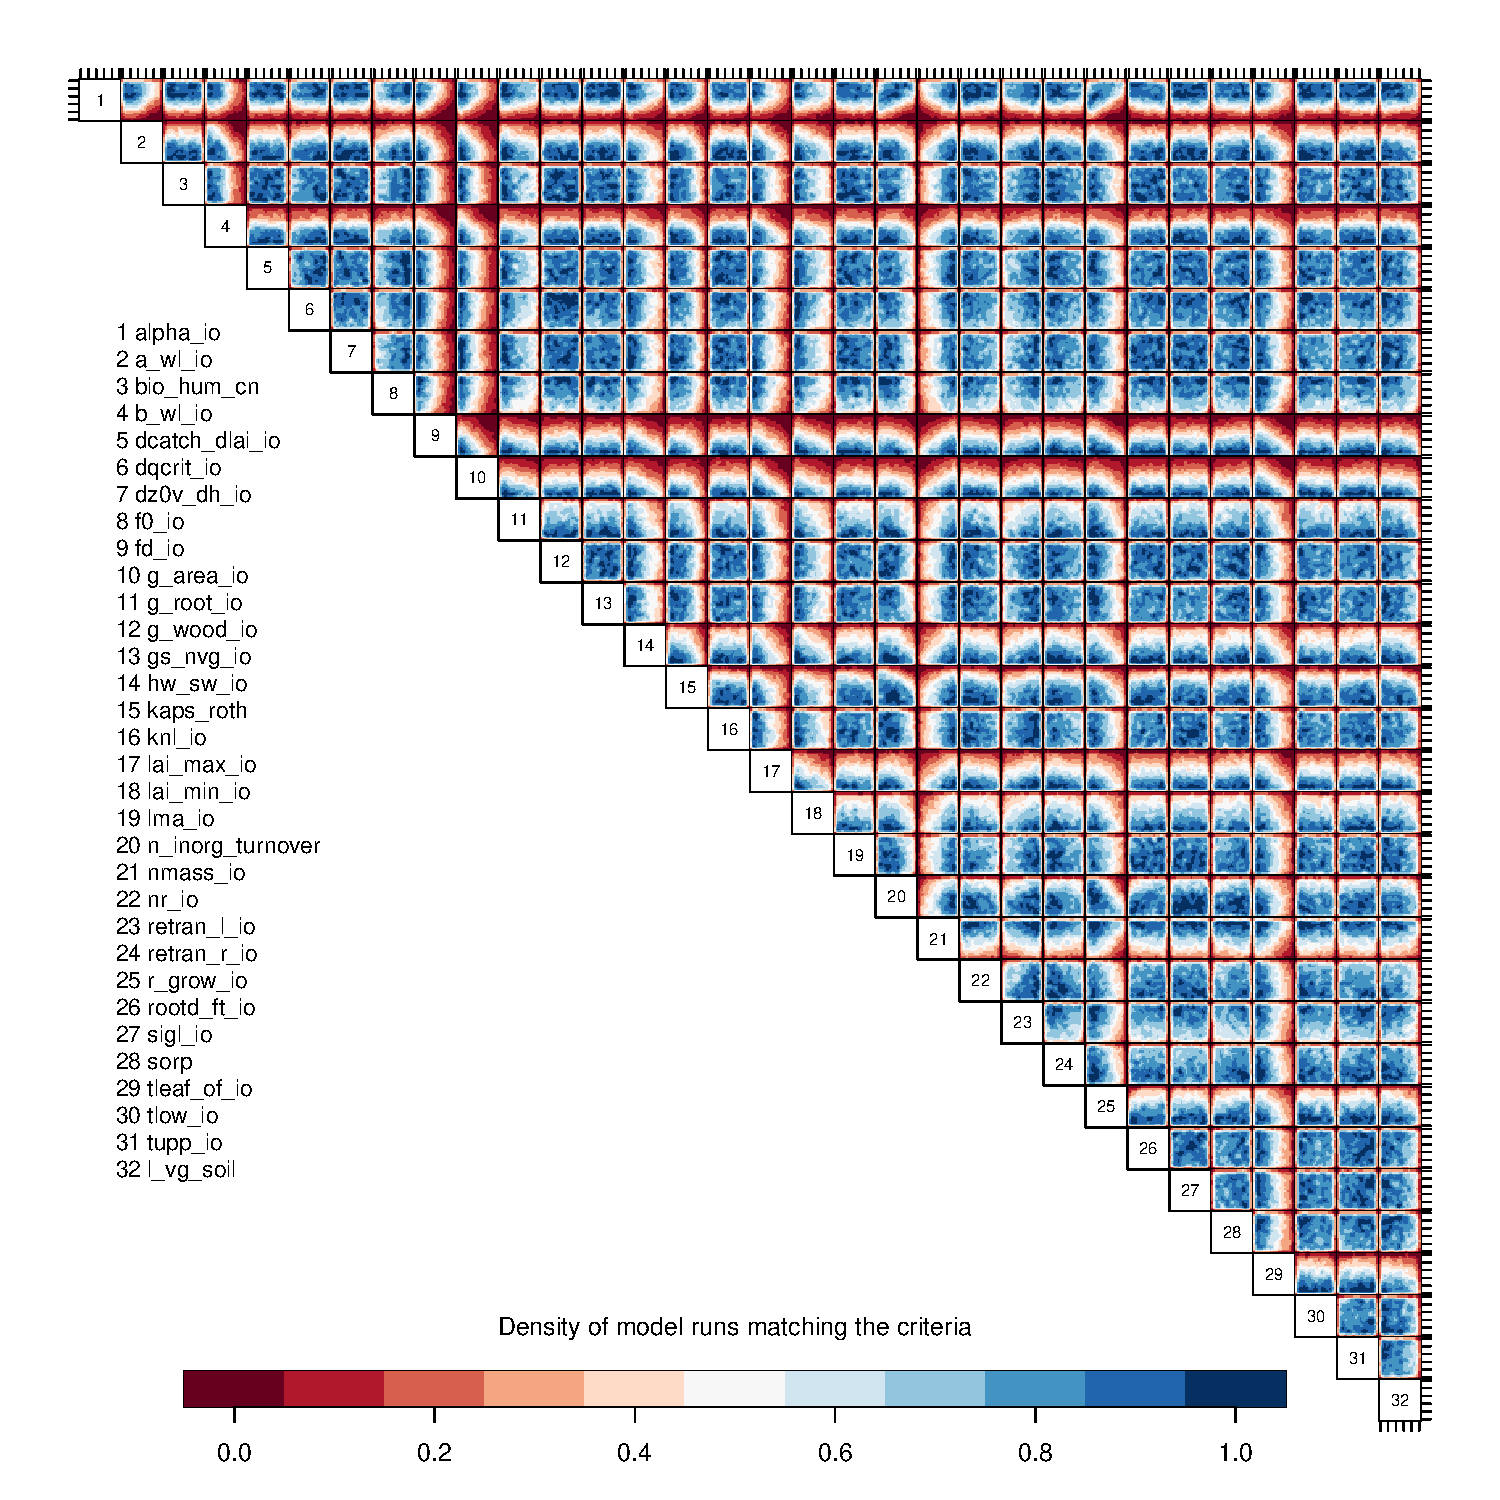
\includegraphics[width=12cm]{./graphics/pairs_dens_level2_km.pdf}
\caption{level 2 pairs density plot}
\label{fig:pairs_dens_level1a_km}
\end{figure*}





%%% TWO-COLUMN FIGURES
%
%%f
\begin{figure*}[t]
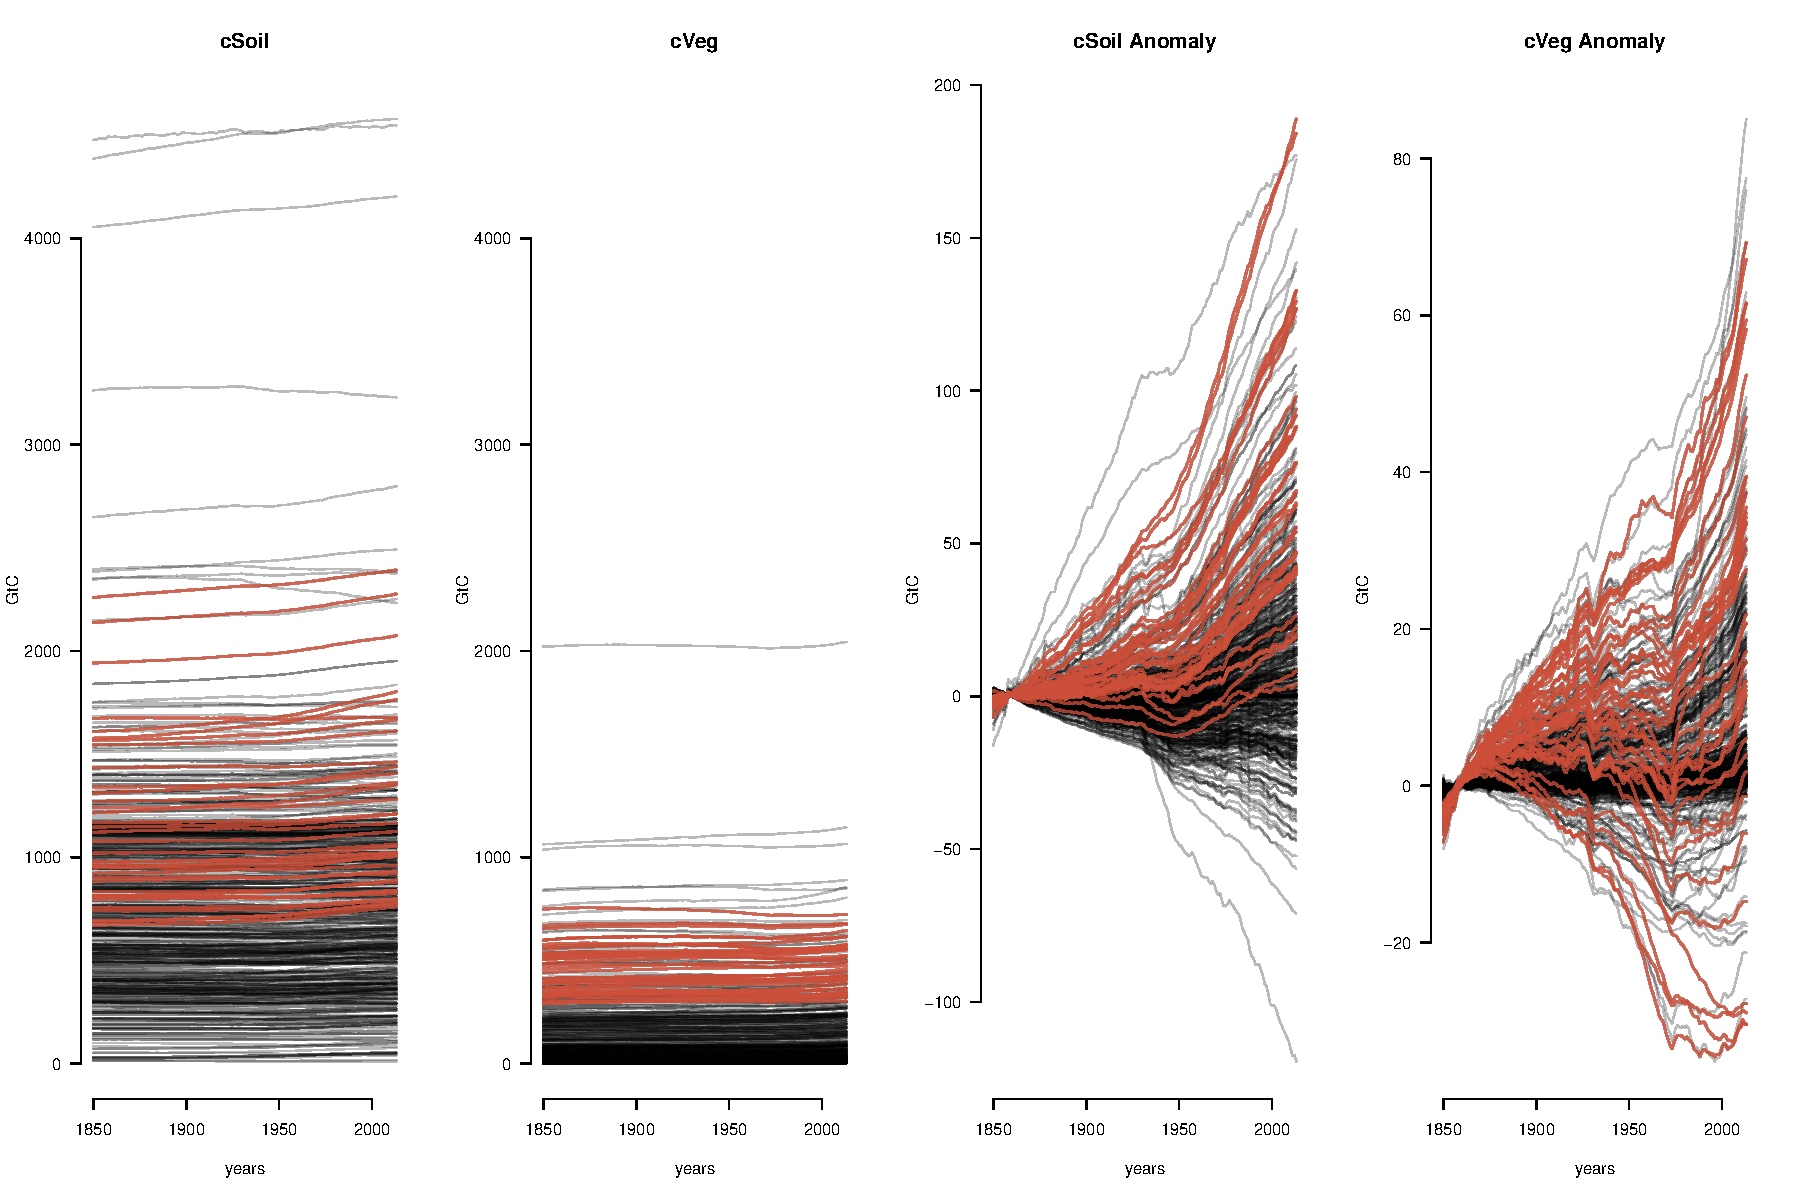
\includegraphics[width=12cm]{./graphics/vegC-soilC-constrained.pdf}
\caption{Constraint of historical soil carbon and vegetation carbon pools}
\label{fig:vegC-soilC-constrained}
\end{figure*}

%%% TWO-COLUMN FIGURES


\subsubsection{Cumulative NBP constraint}

It turns out that constraining with cumulative NBP, and comparing to the AR6 spread does not constrain anywhere near as hard as AW's basic constraints.

\begin{figure*}[t]
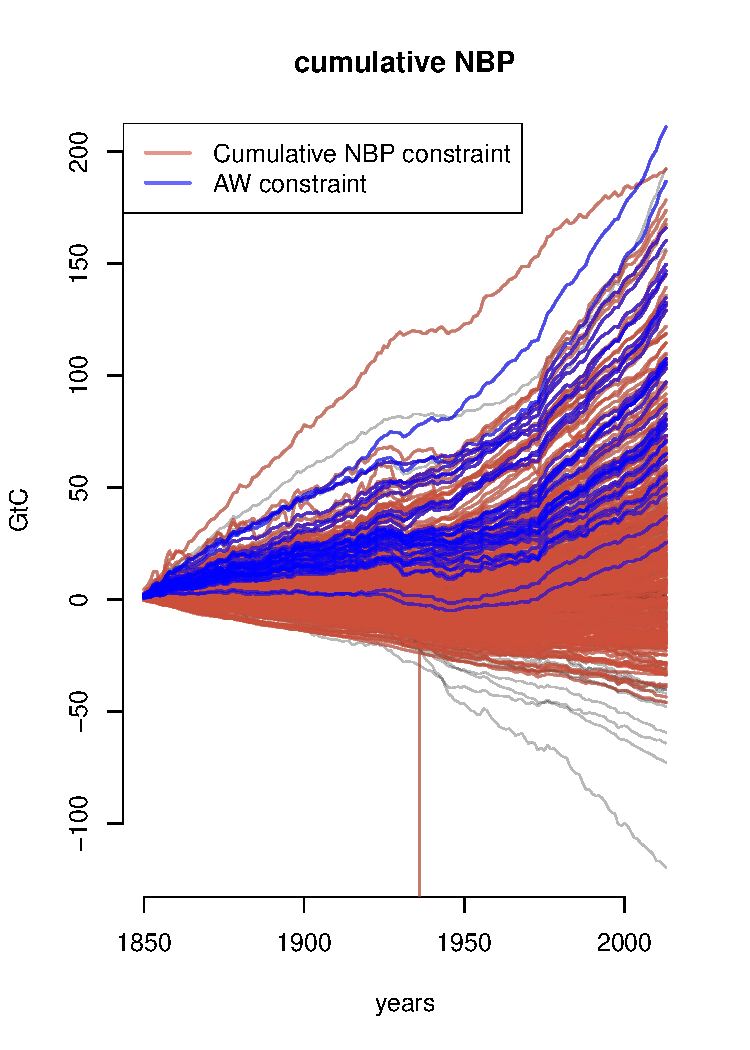
\includegraphics[width=12cm]{./graphics/cumulative_nbp_constrained.pdf}
\caption{Constraint of historical total land carbon pools (veg + soil)}
\label{fig:total-land-carbon-sink-1}
\end{figure*}

\begin{figure*}[t]
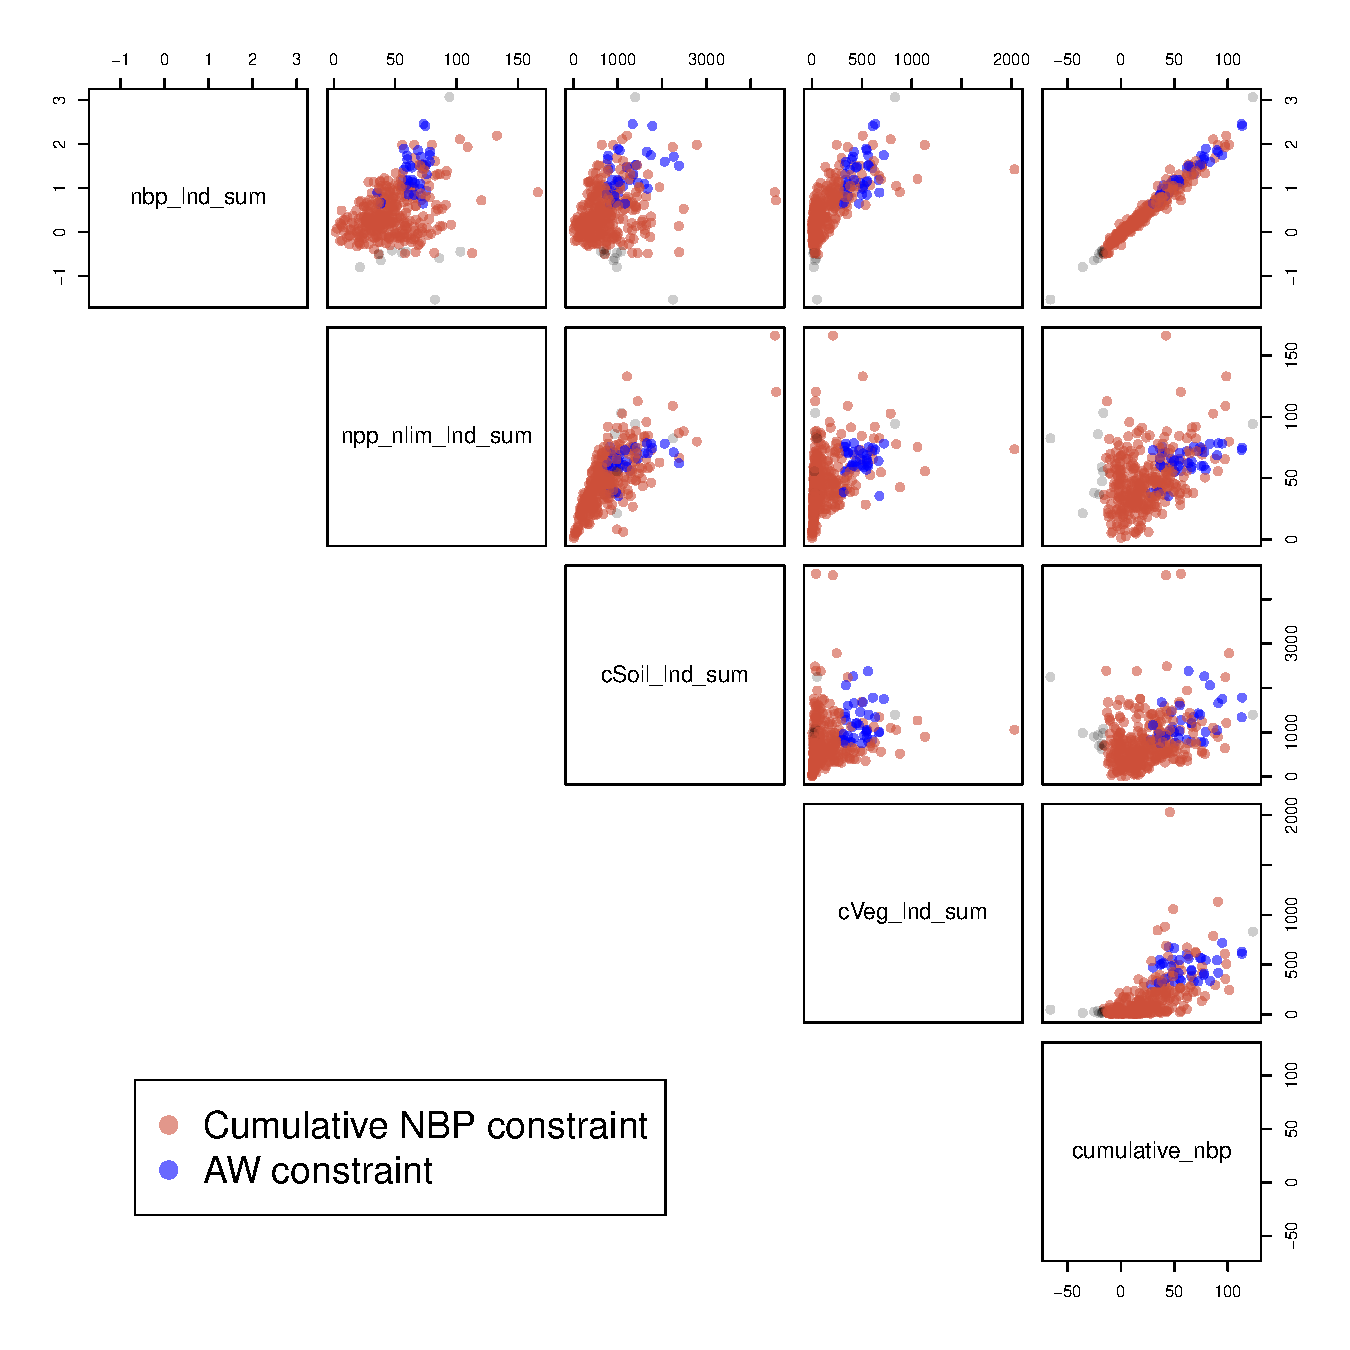
\includegraphics[width=12cm]{./graphics/cumulative_nbp_constrained_pairs.pdf}
\caption{Constraint of historical total land carbon pools (veg + soil)}
\label{fig:total-land-carbon-sink-1}
\end{figure*}
[]

\section{HEADING}
TEXT


\subsection{HEADING}
TEXT


\subsubsection{HEADING}
TEXT


\conclusions  %% \conclusions[modified heading if necessary]
TEXT

%% The following commands are for the statements about the availability of data sets and/or software code corresponding to the manuscript.
%% It is strongly recommended to make use of these sections in case data sets and/or software code have been part of your research the article is based on.

\codeavailability{TEXT} %% use this section when having only software code available


\dataavailability{TEXT} %% use this section when having only data sets available


\codedataavailability{TEXT} %% use this section when having data sets and software code available


\sampleavailability{TEXT} %% use this section when having geoscientific samples available


\videosupplement{TEXT} %% use this section when having video supplements available


\appendix
\section{How good is the emulator?}    %% Appendix A

We assess the quality of the Gaussian Process emulator, for a number of outputs that we use for constraining the parameters of JULES.

Although there are a large number of possible metrics  for validating emualators (see https://core.ac.uk/download/pdf/153535018.pdf), we prefer those that give the modeller as far as possible about the performance of the emulator in terms of the output of the model. As such, we wish to relate the performance directly to the model output. Although the uncertainty of the emulator is important, it takes a secondary role to the performance of the mean prediction.

\subsection{Leave-one-out metrics}     %% Appendix A1, A2, etc.

We use a leave-one-out prediction metric to initially assess the quality of our Gaussian Process emulator. Each of the 362 ensemble members which form the "level 1a" constrained ensemble is removed in turn. A Gaussian Process emulator is trained in its absence and then the withheld ensemble member is predicted. Figure \ref{fig:kmloostats_Ylevel1a} shows a summary plot of the actual value against the predicted value (the mean of the Gaussian process), and associated uncertainty (+- 2 standard deviations), for each output. For each output, we include a summary of the performance across the ensemble in the form of the "proportional mean absolute error (PMAE)", which we define as the mean absolute error of predictaion, when that error is expressed as a fraction of the range of the ensemble.

We find that the PMAE ranges from between around 4\% and around 8\% of the range of the ensemble, with the emulator for cSoil\_lnd\_sum performing best (pmae=3.6\%), and c4PFTfrac\_lnd\_sum performing worst (pmae  8.23\%).

As useful as a summary metric is, it is not the whole story. Some emulators perform 


%%% TWO-COLUMN FIGURES
%
%%f
\begin{figure*}[t]
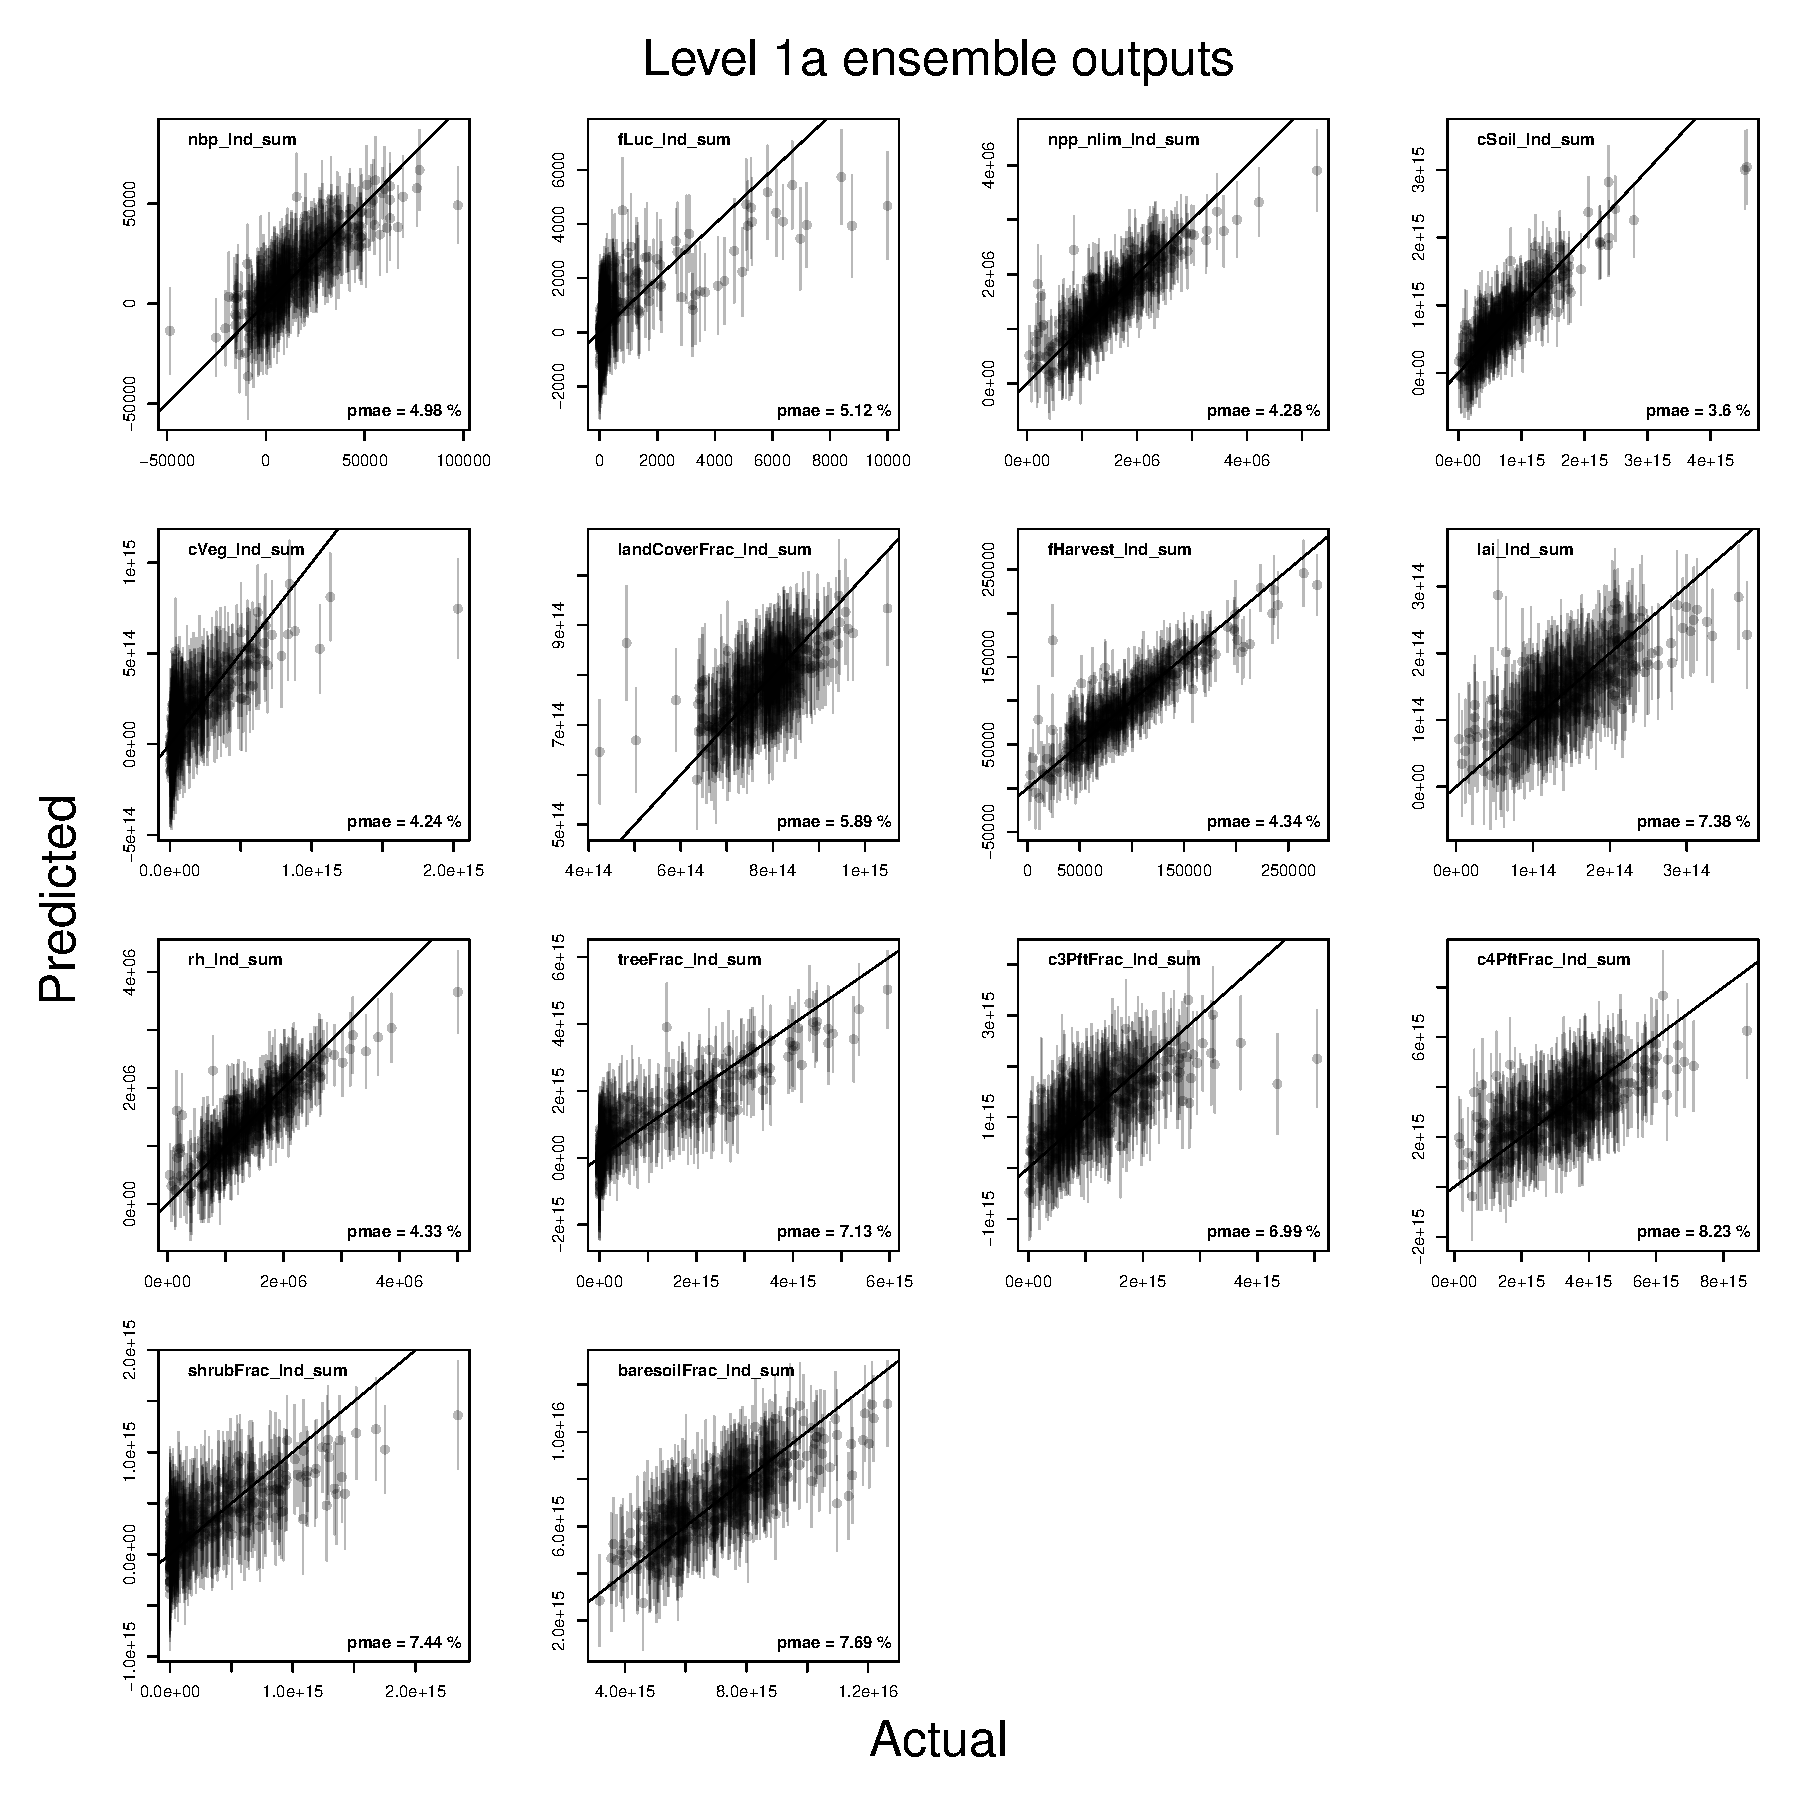
\includegraphics[width=12cm]{./graphics/kmloostats_Ylevel1a.pdf}
\caption{Leave-one-out summaries }
\label{fig:kmloostats_Ylevel1a}
\end{figure*}



\noappendix       %% use this to mark the end of the appendix section. Otherwise the figures might be numbered incorrectly (e.g. 10 instead of 1).

%% Regarding figures and tables in appendices, the following two options are possible depending on your general handling of figures and tables in the manuscript environment:

%% Option 1: If you sorted all figures and tables into the sections of the text, please also sort the appendix figures and appendix tables into the respective appendix sections.
%% They will be correctly named automatically.

%% Option 2: If you put all figures after the reference list, please insert appendix tables and figures after the normal tables and figures.
%% To rename them correctly to A1, A2, etc., please add the following commands in front of them:

\appendixfigures  %% needs to be added in front of appendix figures

\appendixtables   %% needs to be added in front of appendix tables

%% Please add \clearpage between each table and/or figure. Further guidelines on figures and tables can be found below.



\authorcontribution{TEXT} %% this section is mandatory

\competinginterests{TEXT} %% this section is mandatory even if you declare that no competing interests are present

\disclaimer{TEXT} %% optional section

\begin{acknowledgements}
TEXT
\end{acknowledgements}




%% REFERENCES

%% The reference list is compiled as follows:

\begin{thebibliography}{}

\bibitem[AUTHOR(YEAR)]{LABEL1}
REFERENCE 1

\bibitem[AUTHOR(YEAR)]{LABEL2}
REFERENCE 2

\end{thebibliography}

%% Since the Copernicus LaTeX package includes the BibTeX style file copernicus.bst,
%% authors experienced with BibTeX only have to include the following two lines:
%%
%% \bibliographystyle{copernicus}
%% \bibliography{example.bib}
%%
%% URLs and DOIs can be entered in your BibTeX file as:
%%
%% URL = {http://www.xyz.org/~jones/idx_g.htm}
%% DOI = {10.5194/xyz}


%% LITERATURE CITATIONS
%%
%% command                        & example result
%% \citet{jones90}|               & Jones et al. (1990)
%% \citep{jones90}|               & (Jones et al., 1990)
%% \citep{jones90,jones93}|       & (Jones et al., 1990, 1993)
%% \citep[p.~32]{jones90}|        & (Jones et al., 1990, p.~32)
%% \citep[e.g.,][]{jones90}|      & (e.g., Jones et al., 1990)
%% \citep[e.g.,][p.~32]{jones90}| & (e.g., Jones et al., 1990, p.~32)
%% \citeauthor{jones90}|          & Jones et al.
%% \citeyear{jones90}|            & 1990



%% FIGURES

%% When figures and tables are placed at the end of the MS (article in one-column style), please add \clearpage
%% between bibliography and first table and/or figure as well as between each table and/or figure.

% The figure files should be labelled correctly with Arabic numerals (e.g. fig01.jpg, fig02.png).


%% ONE-COLUMN FIGURES

%%f
%\begin{figure}[t]
%\includegraphics[width=8.3cm]{FILE NAME}
%\caption{TEXT}
%\end{figure}
%
%%% TWO-COLUMN FIGURES
%
%%f
%\begin{figure*}[t]
%\includegraphics[width=12cm]{FILE NAME}
%\caption{TEXT}
%\end{figure*}
%
%
%%% TABLES
%%%
%%% The different columns must be seperated with a & command and should
%%% end with \\ to identify the column brake.
%
%%% ONE-COLUMN TABLE
%
%%t
%\begin{table}[t]
%\caption{TEXT}
%\begin{tabular}{column = lcr}
%\tophline
%
%\middlehline
%
%\bottomhline
%\end{tabular}
%\belowtable{} % Table Footnotes
%\end{table}
%
%%% TWO-COLUMN TABLE
%
%%t
%\begin{table*}[t]
%\caption{TEXT}
%\begin{tabular}{column = lcr}
%\tophline
%
%\middlehline
%
%\bottomhline
%\end{tabular}
%\belowtable{} % Table Footnotes
%\end{table*}
%
%%% LANDSCAPE TABLE
%
%%t
%\begin{sidewaystable*}[t]
%\caption{TEXT}
%\begin{tabular}{column = lcr}
%\tophline
%
%\middlehline
%
%\bottomhline
%\end{tabular}
%\belowtable{} % Table Footnotes
%\end{sidewaystable*}
%
%
%%% MATHEMATICAL EXPRESSIONS
%
%%% All papers typeset by Copernicus Publications follow the math typesetting regulations
%%% given by the IUPAC Green Book (IUPAC: Quantities, Units and Symbols in Physical Chemistry,
%%% 2nd Edn., Blackwell Science, available at: http://old.iupac.org/publications/books/gbook/green_book_2ed.pdf, 1993).
%%%
%%% Physical quantities/variables are typeset in italic font (t for time, T for Temperature)
%%% Indices which are not defined are typeset in italic font (x, y, z, a, b, c)
%%% Items/objects which are defined are typeset in roman font (Car A, Car B)
%%% Descriptions/specifications which are defined by itself are typeset in roman font (abs, rel, ref, tot, net, ice)
%%% Abbreviations from 2 letters are typeset in roman font (RH, LAI)
%%% Vectors are identified in bold italic font using \vec{x}
%%% Matrices are identified in bold roman font
%%% Multiplication signs are typeset using the LaTeX commands \times (for vector products, grids, and exponential notations) or \cdot
%%% The character * should not be applied as mutliplication sign
%
%
%%% EQUATIONS
%
%%% Single-row equation
%
%\begin{equation}
%
%\end{equation}
%
%%% Multiline equation
%
%\begin{align}
%& 3 + 5 = 8\\
%& 3 + 5 = 8\\
%& 3 + 5 = 8
%\end{align}
%
%
%%% MATRICES
%
%\begin{matrix}
%x & y & z\\
%x & y & z\\
%x & y & z\\
%\end{matrix}
%
%
%%% ALGORITHM
%
%\begin{algorithm}
%\caption{...}
%\label{a1}
%\begin{algorithmic}
%...
%\end{algorithmic}
%\end{algorithm}
%
%
%%% CHEMICAL FORMULAS AND REACTIONS
%
%%% For formulas embedded in the text, please use \chem{}
%
%%% The reaction environment creates labels including the letter R, i.e. (R1), (R2), etc.
%
%\begin{reaction}
%%% \rightarrow should be used for normal (one-way) chemical reactions
%%% \rightleftharpoons should be used for equilibria
%%% \leftrightarrow should be used for resonance structures
%\end{reaction}
%
%
%%% PHYSICAL UNITS
%%%
%%% Please use \unit{} and apply the exponential notation


\end{document}
